% Options for packages loaded elsewhere
\PassOptionsToPackage{unicode}{hyperref}
\PassOptionsToPackage{hyphens}{url}
\PassOptionsToPackage{dvipsnames,svgnames*,x11names*}{xcolor}
%
\documentclass[
  a4paper,
  openany, a4paper, oneside]{book}
\usepackage{amsmath,amssymb}
\usepackage{lmodern}
\usepackage{setspace}
\usepackage{ifxetex,ifluatex}
\ifnum 0\ifxetex 1\fi\ifluatex 1\fi=0 % if pdftex
  \usepackage[T1]{fontenc}
  \usepackage[utf8]{inputenc}
  \usepackage{textcomp} % provide euro and other symbols
\else % if luatex or xetex
  \usepackage{unicode-math}
  \defaultfontfeatures{Scale=MatchLowercase}
  \defaultfontfeatures[\rmfamily]{Ligatures=TeX,Scale=1}
\fi
% Use upquote if available, for straight quotes in verbatim environments
\IfFileExists{upquote.sty}{\usepackage{upquote}}{}
\IfFileExists{microtype.sty}{% use microtype if available
  \usepackage[]{microtype}
  \UseMicrotypeSet[protrusion]{basicmath} % disable protrusion for tt fonts
}{}
\makeatletter
\@ifundefined{KOMAClassName}{% if non-KOMA class
  \IfFileExists{parskip.sty}{%
    \usepackage{parskip}
  }{% else
    \setlength{\parindent}{0pt}
    \setlength{\parskip}{6pt plus 2pt minus 1pt}}
}{% if KOMA class
  \KOMAoptions{parskip=half}}
\makeatother
\usepackage{xcolor}
\IfFileExists{xurl.sty}{\usepackage{xurl}}{} % add URL line breaks if available
\IfFileExists{bookmark.sty}{\usepackage{bookmark}}{\usepackage{hyperref}}
\hypersetup{
  pdftitle={Automated Observatory Contributors' Handbook},
  pdfauthor={Daniel Antal, CFA},
  colorlinks=true,
  linkcolor=blue,
  filecolor=Maroon,
  citecolor=Blue,
  urlcolor=blue,
  pdfcreator={LaTeX via pandoc}}
\urlstyle{same} % disable monospaced font for URLs
\usepackage[left=2.5cm, right=2.5cm, top=2.5cm, bottom=2.5cm]{geometry}
\usepackage{longtable,booktabs,array}
\usepackage{calc} % for calculating minipage widths
% Correct order of tables after \paragraph or \subparagraph
\usepackage{etoolbox}
\makeatletter
\patchcmd\longtable{\par}{\if@noskipsec\mbox{}\fi\par}{}{}
\makeatother
% Allow footnotes in longtable head/foot
\IfFileExists{footnotehyper.sty}{\usepackage{footnotehyper}}{\usepackage{footnote}}
\makesavenoteenv{longtable}
\usepackage{graphicx}
\makeatletter
\def\maxwidth{\ifdim\Gin@nat@width>\linewidth\linewidth\else\Gin@nat@width\fi}
\def\maxheight{\ifdim\Gin@nat@height>\textheight\textheight\else\Gin@nat@height\fi}
\makeatother
% Scale images if necessary, so that they will not overflow the page
% margins by default, and it is still possible to overwrite the defaults
% using explicit options in \includegraphics[width, height, ...]{}
\setkeys{Gin}{width=\maxwidth,height=\maxheight,keepaspectratio}
% Set default figure placement to htbp
\makeatletter
\def\fps@figure{htbp}
\makeatother
\setlength{\emergencystretch}{3em} % prevent overfull lines
\providecommand{\tightlist}{%
  \setlength{\itemsep}{0pt}\setlength{\parskip}{0pt}}
\setcounter{secnumdepth}{5}
\usepackage{booktabs}
\ifluatex
  \usepackage{selnolig}  % disable illegal ligatures
\fi
\usepackage[]{natbib}
\bibliographystyle{apalike}

\title{Automated Observatory Contributors' Handbook}
\author{Daniel Antal, CFA}
\date{2021-06-21}

\begin{document}
\maketitle

{
\hypersetup{linkcolor=}
\setcounter{tocdepth}{1}
\tableofcontents
}
\listoffigures
\setstretch{1.1}
\hypertarget{introduction}{%
\chapter*{Introduction}\label{introduction}}
\addcontentsline{toc}{chapter}{Introduction}

If open data is the new gold, why even those who release fail to reuse it? We created an open collaboration of data curators and open-source developers to dig into novel open data sources or increase the usability of existing ones. We turn reproducible research software into research- as-service.

Reprex, a Dutch start-up enterprise formed to utilize open source software and open data, is looking for partners in an agile, open collaboration to win at least one of the three EU Datathon Prizes. We are looking for policy partners, academic partners and a consultancy partner. Our project is based on agile, open collaboration with three types of contributors.

\begin{itemize}
\item
  \emph{To take part, you should propose the development of an application that links and uses open datasets.} - we are curating new, exciting \protect\hyperlink{data-domains}{data sources}, that are legally open but usually have never seen the sunlight.
\item
  \emph{Your application \ldots{} is also expected to find suitable new approaches and solutions to help Europe achieve important goals set by the European Commission through the use of open data.}'' - we have a prototype of this \protect\hyperlink{tech-solution}{application}
\item
  \emph{Your application should showcase opportunities for concrete business models or social enterprises.} - our \protect\hyperlink{business-solution}{service development team} is working to make this happen!
\end{itemize}

We believe in \href{}{open collaboration} that involves \protect\hyperlink{intro-academic-partners}{scientific}, \protect\hyperlink{intro-business-partners}{business}, public and NGO \protect\hyperlink{intro-policy-partners}{policy} partnerships.

\hypertarget{whatss-wrong-with-open-data}{%
\section*{1. Whats's Wrong With Open Data?}\label{whatss-wrong-with-open-data}}
\addcontentsline{toc}{section}{1. Whats's Wrong With Open Data?}

Open data is like gold in the mud below the chilly waves of mountain rivers. Panning it out requires a lot of patience, or a good machine. I think we will come to as surprising and strong findings as Bellingcat, but we are not focusing on individual events and stories, but on social and environmental processes and changes.

\begin{center}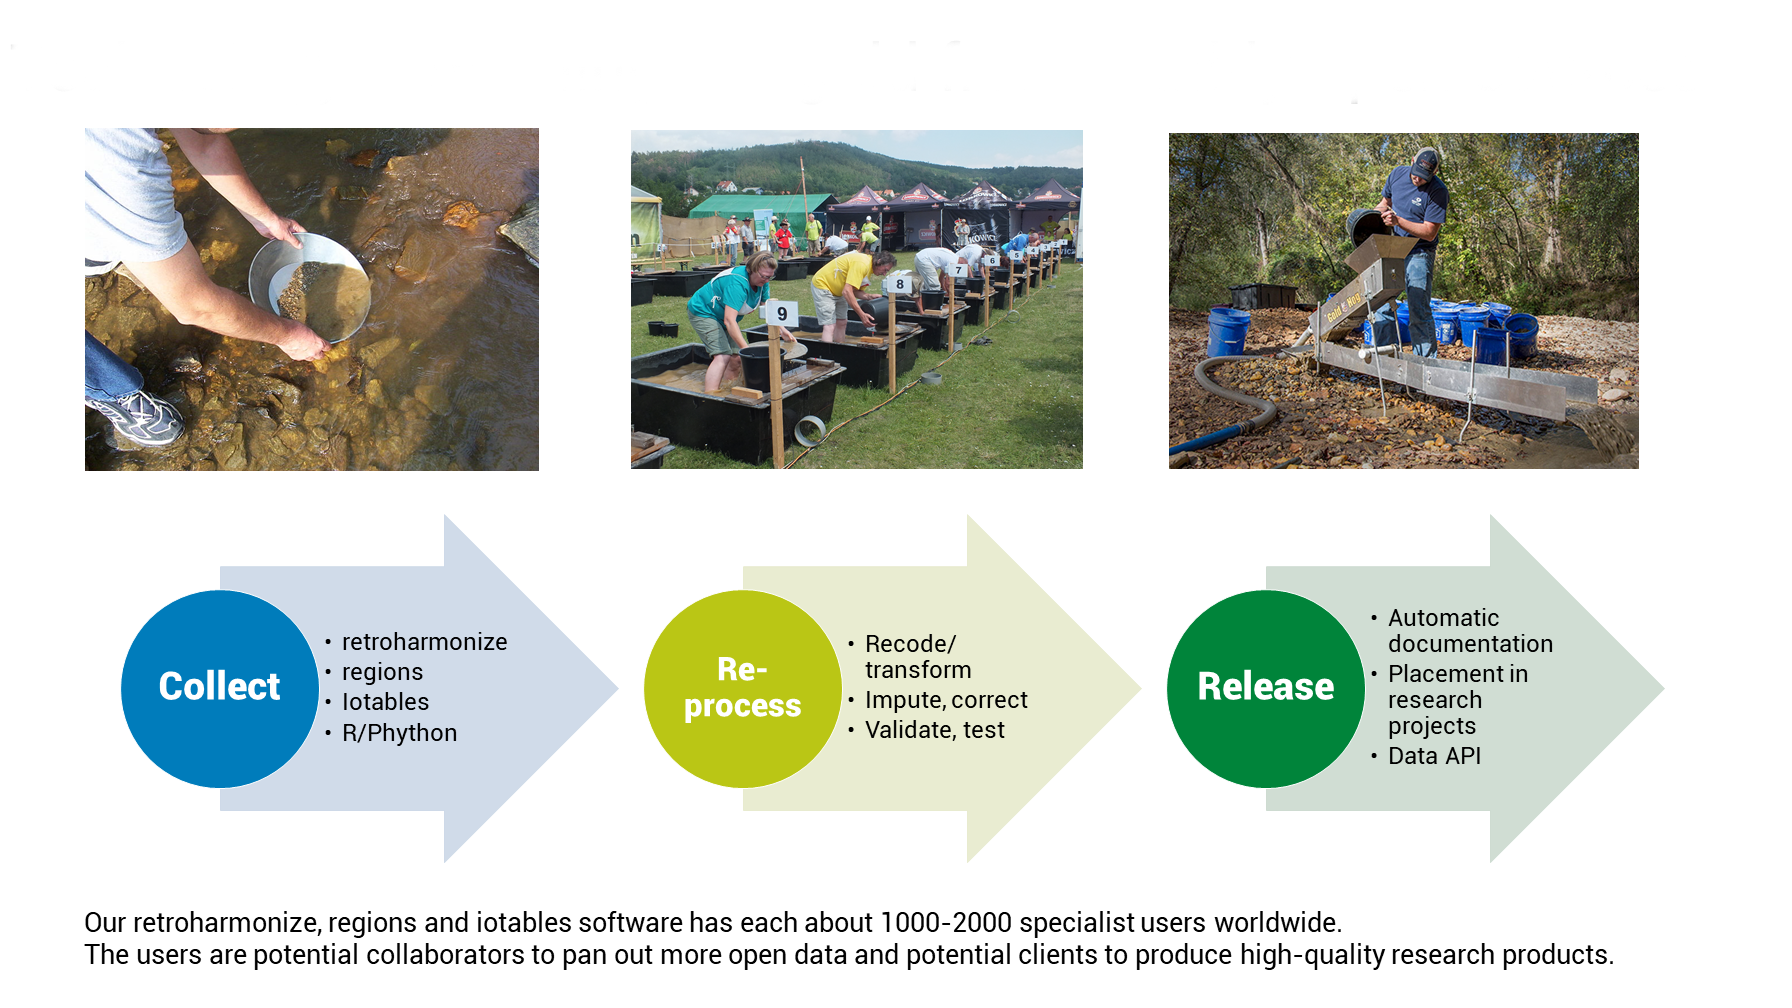
\includegraphics[width=24.89in]{C:/_bookdown/observatory_data_curators/plots/slides/gold_panning_slide_notitle} \end{center}

In \ref{open-data} \protect\hyperlink{open-data}{Open Data} we investigate why not even those organizations, like the European Commission, use open data in their own data dissemination practices, who make them at least legally available.

\hypertarget{tech-solution}{%
\section*{2. Our Technological Solution}\label{tech-solution}}
\addcontentsline{toc}{section}{2. Our Technological Solution}

We use open source software and open data. The applications are hosted on the cloud resources of \protect\hyperlink{reprex}{Reprex}, an early-stage technology startup currently building a viable, open-source, open-data business model to create reproducible research products.

Our development team works on an open collaboration basis. Our indicator R packages, and our services are developed together with \href{https://music.dataobservatory.eu/author/ropengov/}{rOpenGov}.

\begin{itemize}
\tightlist
\item
  Open data often cannot be downloaded.
\item
  Open data often lacks quality control.
\item
  Public data sources are not tidy.
\item
  The risk of importing or committing trivial data processing errors is huge.
\item
  Open data is usually not documented.
\end{itemize}

See \ref{app}. \protect\hyperlink{app}{Application: Automated Data Observatories} for further details.

\hypertarget{business-solution}{%
\section*{3. Our Business Solution}\label{business-solution}}
\addcontentsline{toc}{section}{3. Our Business Solution}

We decided to take a new, modern approach to the `data observatory' concept, and modernize it with the application of 21st century data and metadata standards, the new results of reproducible research and data science. Various UN and OECD bodies, and particularly the European Union support or maintain more than 60 data observatories, or permanent data collection and dissemination points, but even these do not use these organizations and their members open data.

We are building open-source data observatories, which run open-source statistical software that automatically processes and documents reusable public sector data (from public transport, meteorology, tax offices, taxpayer funded satellite systems, etc.) and reusable scientific data (from EU taxpayer funded research) into new, high quality statistical indicators.

Our Product/Market Fit was validated in the world's 2nd ranked university-backed incubator program, the \href{https://music.dataobservatory.eu/post/2020-09-25-yesdelft-validation/}{Yes!Delft AI Validation Lab}. We are currently developing this project with the help of the \href{https://www.jumpmusic.eu/fellow2021/automated-music-observatory/}{JUMP European Music Market Accelerator} program.

See \ref{service}. \protect\hyperlink{service}{Service Design and Business Case Development}

\hypertarget{open-for-partners}{%
\section*{4. Open Collaboration: Partners and Partnership}\label{open-for-partners}}
\addcontentsline{toc}{section}{4. Open Collaboration: Partners and Partnership}

We are looking for partners to develop our \protect\hyperlink{app}{technological solution} in \href{service}{financially sustainable way} with bringing more and more relevant, \protect\hyperlink{data-curators}{curated} open data \protect\hyperlink{open-data}{to light}.

\hypertarget{intro-academic-partners}{%
\subsection*{Academic partners}\label{intro-academic-partners}}
\addcontentsline{toc}{subsection}{Academic partners}

We are looking for academic partners who want to use open data from various governmental (including publicly funded surveys), scientific, and big data sources, processed and validated to meet scientific standards. We provide peer-reviewed statistical software solutions, daily data harvesting, and re-processing to meet our partners research agenda. See more in \ref{academic-partners} \protect\hyperlink{academic-partners}{Academic partners}

\hypertarget{intro-policy-partners}{%
\subsection*{Policy partners}\label{intro-policy-partners}}
\addcontentsline{toc}{subsection}{Policy partners}

We are looking for policy partners who want to use open data from various governmental (including publicly funded surveys), scientific, and big data sources, processed and validated to meet scientific standards; or who want to build use cases for trustworthy AI and data governance policy papers. We provide peer-reviewed statistical software solutions, daily data harvesting, and re-processing to meet our partners' research agenda. See more in \ref{policy-partners} \protect\hyperlink{policy-partners}{Policy partners}

\hypertarget{intro-business-partners}{%
\subsection*{Business partner(s) in Consulting}\label{intro-business-partners}}
\addcontentsline{toc}{subsection}{Business partner(s) in Consulting}

We are looking for a consulting partner to form a joint project with our open collaboration team of data scientists and submit proposals to at least 2 of the 3 challenges of the EU Datathlon with the objective of winning the first prize. We are particularly looking for a first class consultancy to help build a ``showcase \ldots{} for concrete business models {[}\ldots{} and{]} find suitable new approaches and solutions to help Europe achieve important goals set by the European Commission through the use of {[}our observatories'{]} open data.'' See more in \ref{business-partners} \protect\hyperlink{business-partners}{Business partners}

\hypertarget{data-domains}{%
\section*{5. Data Domains}\label{data-domains}}
\addcontentsline{toc}{section}{5. Data Domains}

\begin{itemize}
\tightlist
\item
  We are working together with experts in the domain as curators (check out our guidelines if you want to join: \href{https://curators.dataobservatory.eu/data-curators.html}{Data Curators: Get Inspired!}).
\end{itemize}

\hypertarget{green-deal-data-observaotry}{%
\subsection*{Green Deal Data Observaotry}\label{green-deal-data-observaotry}}
\addcontentsline{toc}{subsection}{Green Deal Data Observaotry}

The Challenge \href{https://ec.europa.eu/info/strategy/priorities-2019-2024/european-green-deal_en}{A European Green Deal}, with a particular focus on the \href{https://ec.europa.eu/commission/presscorner/detail/en/ip_20_2323}{The European Climate Pact}, the \href{https://ec.europa.eu/info/food-farming-fisheries/farming/organic-farming/organic-action-plan_en}{Organic Action Plan}, and the \href{https://ec.europa.eu/commission/presscorner/detail/en/IP_21_111}{New European Bauhaus}, i.e., mitigation strategies. Our \href{http://greendeal.dataobservatory.eu/}{Green Deal Data Observatory} is a modern reimagination of existing `data observatories'; currently, there are over 70 permanent international data collection and dissemination points. One of our objectives is to understand why the dozens of the EU's observatories do not use open data and reproducible research. We want to show that open governmental data, open science, and reproducible research can lead to a higher quality and faster data ecosystem that fosters growth for policy, business, and academic data users.

\begin{center}\includegraphics[width=26.32in]{C:/_bookdown/observatory_data_curators/plots/screenshots/greendeal_and_zenodo} \end{center}

Please, follow us on social media, it really helps us finding new users and showing that we are able to grow our ecosystem: the \href{https://www.linkedin.com/company/78556699}{Green Deal Data Observatory on Linkedin} and the \href{https://twitter.com/GreenDealObs}{Green Deal Data Observatory on Twitter}, and join our \href{https://greendeal.dataobservatory.eu/\#contributors}{contributor team}.

\hypertarget{digital-music-observatory}{%
\subsection*{Digital Music Observatory}\label{digital-music-observatory}}
\addcontentsline{toc}{subsection}{Digital Music Observatory}

The \href{https://music.dataobservatory.eu/}{Digital Music Observatory} is a fully automated, open source, open data observatory that creates public datasets to provide a comprehensive view of the European music industry. It provides high-quality and timely indicators in all four pillars of the planned official European Music Observatory as a modern, open source and largely open data-based, automated, API-supported alternative solution for this planned observatory. The insight and methodologies we are refining in the DMO are applicable and transferable to about 60 other data observatories funded by the EU which do not currently employ governmental or scientific open data.

See further details in \ref{music} \protect\hyperlink{music}{Digital Music Observatory Chapter}.

\begin{center}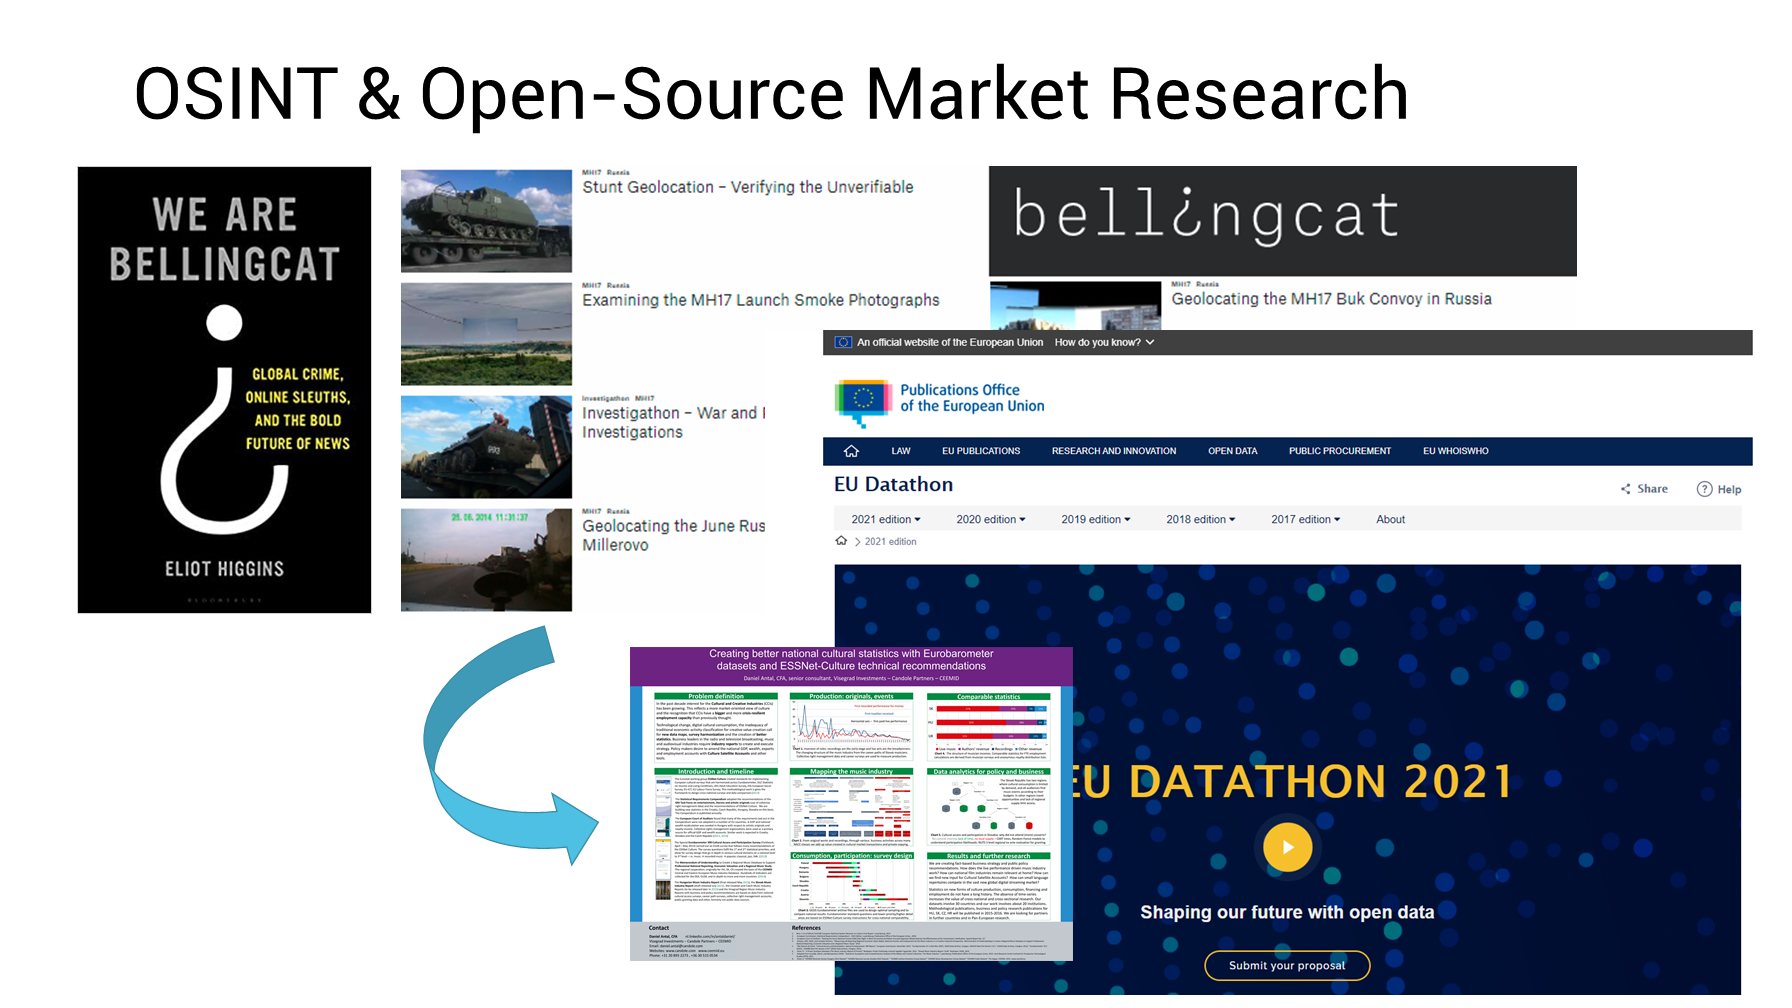
\includegraphics[width=24.89in]{C:/_bookdown/observatory_data_curators/plots/slides/open_source_slide} \end{center}

Please, follow us on social media, it really helps us finding new users and showing that we are able to grow our ecosystem: the \href{https://www.linkedin.com/company/79286750/}{Digital Music Data Observatory on Linkedin} and the \href{https://twitter.com/DigitalMusicObs}{Digital Music Data Observatory on Twitter} and join our \href{https://music.dataobservatory.eu/\#contributors}{contributor team}.

\hypertarget{economy-data-observatory}{%
\subsection*{Economy Data Observatory}\label{economy-data-observatory}}
\addcontentsline{toc}{subsection}{Economy Data Observatory}

Our \href{https://economy.dataobservatory.eu/}{Economy Data Observatory} was created as a prototype for the EU Datathon Challenge 2: \href{https://ec.europa.eu/info/strategy/priorities-2019-2024/economy-works-people_en\#:~:text=Individuals\%20and\%20businesses\%20in\%20the,needs\%20of\%20the\%20EU's\%20citizens.}{An economy that works for people}, with a particular focus on the \href{https://ec.europa.eu/info/strategy/priorities-2019-2024/economy-works-people/internal-market_en}{Single market strategy}, and particular attention to the strategy's goals of 1. Modernising our standards system, 2. Consolidating Europe's intellectual property framework, and 3. Enabling the balanced development of the collaborative economy strategic goals.

Big data and automation create new inequalities and injustices and have the potential to create a jobless growth economy. Our is a fully automated, open source, open data observatory that produces new indicators from open data sources and experimental big data sources, with authoritative copies and a modern API.

The \href{https://economy.dataobservatory.eu/}{Economy Data Observatory} works now as an incubator for economy-focused data observatories. See further details in \ref{economy} \protect\hyperlink{economy}{Economy Data Observatory Chapter}.

\begin{center}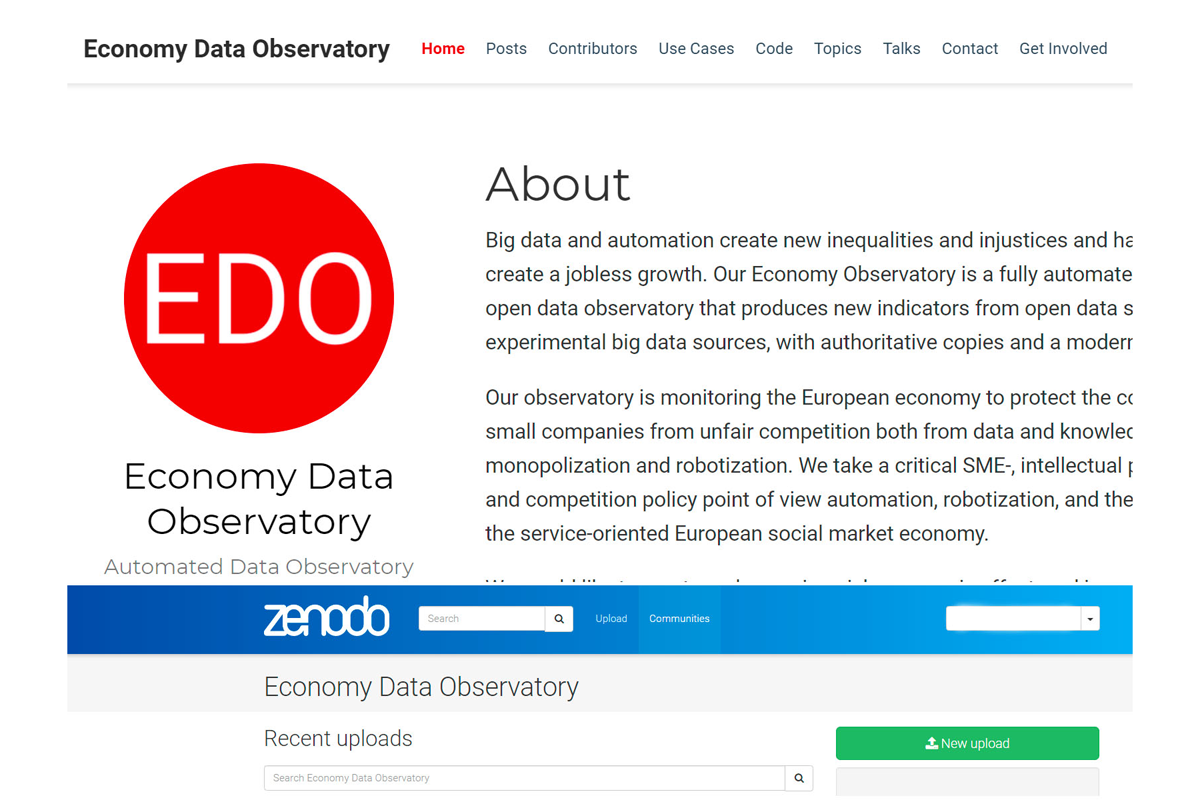
\includegraphics[width=16.67in]{C:/_bookdown/observatory_data_curators/plots/screenshots/edo_and_zenodo} \end{center}

Please, follow us on social media, it really helps us finding new users and showing that we are able to grow our ecosystem: the \href{https://www.linkedin.com/company/78562153/}{Economy Data Observatory on Linkedin} and the \href{https://twitter.com/EconDataObs/}{Economy Data Observatory on Twitter} and join our \href{https://economy.dataobservatory.eu/\#contributors}{contributor team}.

\hypertarget{competition-data-observatory}{%
\subsection*{Competition Data Observatory}\label{competition-data-observatory}}
\addcontentsline{toc}{subsection}{Competition Data Observatory}

The \href{https://competition-data-observatory.netlify.app/}{Competition Data Observatory} is the first offspring of the \href{https://economy.dataobservatory.eu/}{Economy Data Observatory} incubator. See further details in \ref{competition} \protect\hyperlink{competition}{Competition Data Observatory Chapter}.

We would like to create early-warning, risk, economic effect, and impact indicators that can be used in scientific, business and policy contexts for professionals who are working on re-setting the European economy after a devastating pandemic and in the age of AI. We would like to map data between economic activities (NACE), antitrust markets, and sub-national, regional, metropolitian area data.

\begin{center}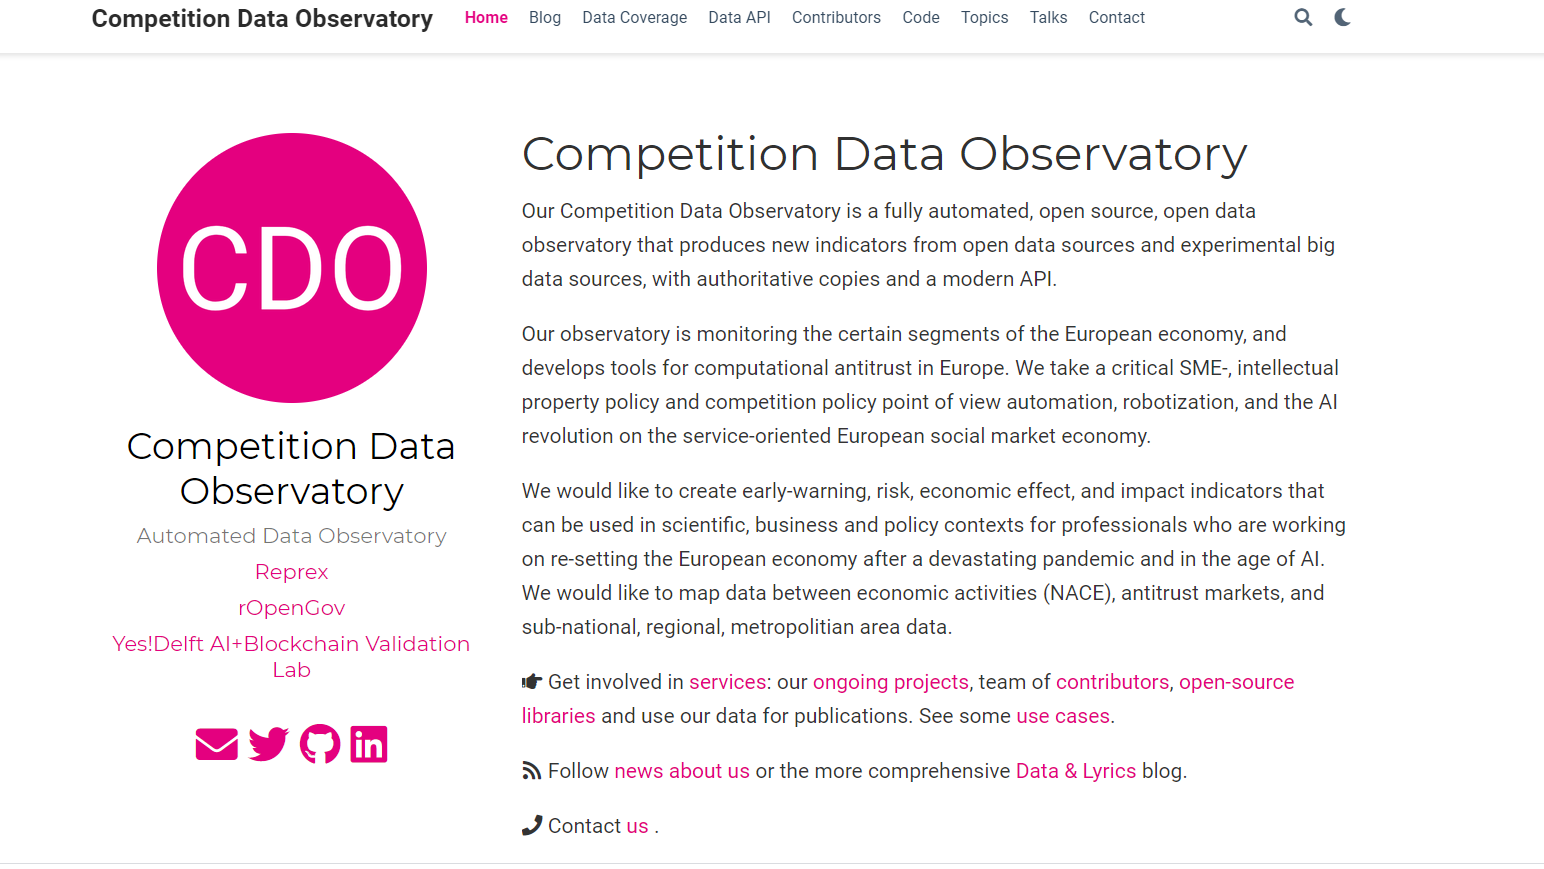
\includegraphics[width=21.44in]{C:/_bookdown/observatory_data_curators/plots/screenshots/cdo_opening_page} \end{center}

\hypertarget{open-data}{%
\chapter{Open Data}\label{open-data}}

In the EU, open data is governed by the \href{https://eur-lex.europa.eu/legal-content/EN/TXT/?qid=1561563110433\&uri=CELEX:32019L1024}{Directive on open data and the re-use of public sector information - in short: Open Data Directive (EU) 2019 / 1024}. It entered into force on 16 July 2019. It replaces the \href{https://eur-lex.europa.eu/legal-content/en/ALL/?uri=CELEX:32003L0098}{Public Sector Information Directive}, also known as the \emph{PSI Directive} which dated from 2003 and was subsequently amended in 2013.

\href{https://greendeal.dataobservatory.eu/post/2021-06-10-founder-daniel-antal/}{Open Data is Like Gold in the Mud Below the Chilly Waves of Mountain Rivers}

The EU has an 18-year-old open data regime and it makes public taxpayer-funded data in the values of tens of billions of euros per year; the Eurostat program alone handles 20,000 international data products, including at least 5,000 pan-European environmental indicators.

As open science principles gain increased acceptance, scientific researchers are making hundreds of thousands of valuable datasets public and available for replication every year.

The EU, the OECD, and UN institutions run around 100 data collection programs, so-called `data observatories' that more or less avoid touching this data, and buy proprietary data instead. Annually, each observatory spends between 50 thousand and 3 million EUR on collecting untidy and proprietary data of inconsistent quality, while never even considering open data.

\begin{center}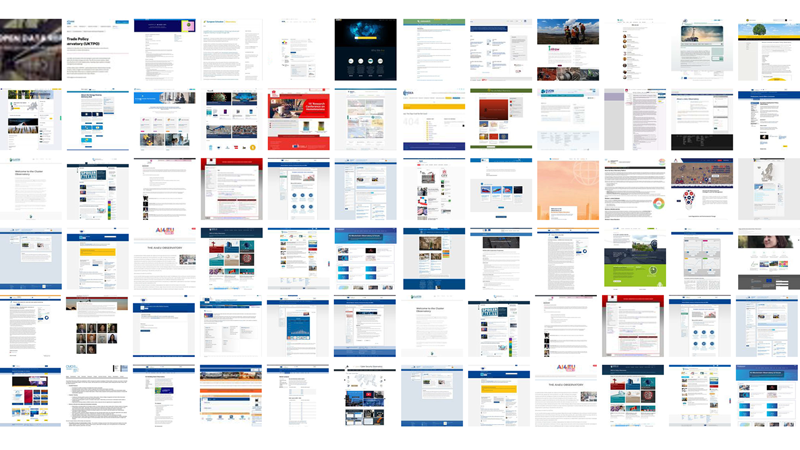
\includegraphics[width=11.11in]{plots/screenshots/observatory_collage_16x9_800} \end{center}

The problem with the current EU data strategy is that while it produces enormous quantities of valuable open data, in the absence of common basic data science and documentation principles, it seems often cheaper to create new data than to put the existing open data into shape.

This is an absolute waste of resources and efforts. With a few R packages and our deep understanding of advanced data science techniques, we can create valuable datasets from unprocessed open data. In most domains, we are able to repurpose data originally created for other purposes at a historical cost of several billions of euros, converting these unused data assets into valuable datasets that can replace tens of millions' worth of proprietary data.

What we want to achieve with this project -- and we believe such an accomplishment would merit one of the first prizes - is to add value to a significant portion of pre-existing EU open data (for example, available on \href{https://data.europa.eu/data/}{data.europa.eu/data}) by re-processing and integrating them into a modern, tidy database with an API access, and to find a business model that emphasises a triangular use of data in 1. business, 2. science and 3. policy-making. Our mission is to modernize the concept of \texttt{data\ observatories.}

\begin{center}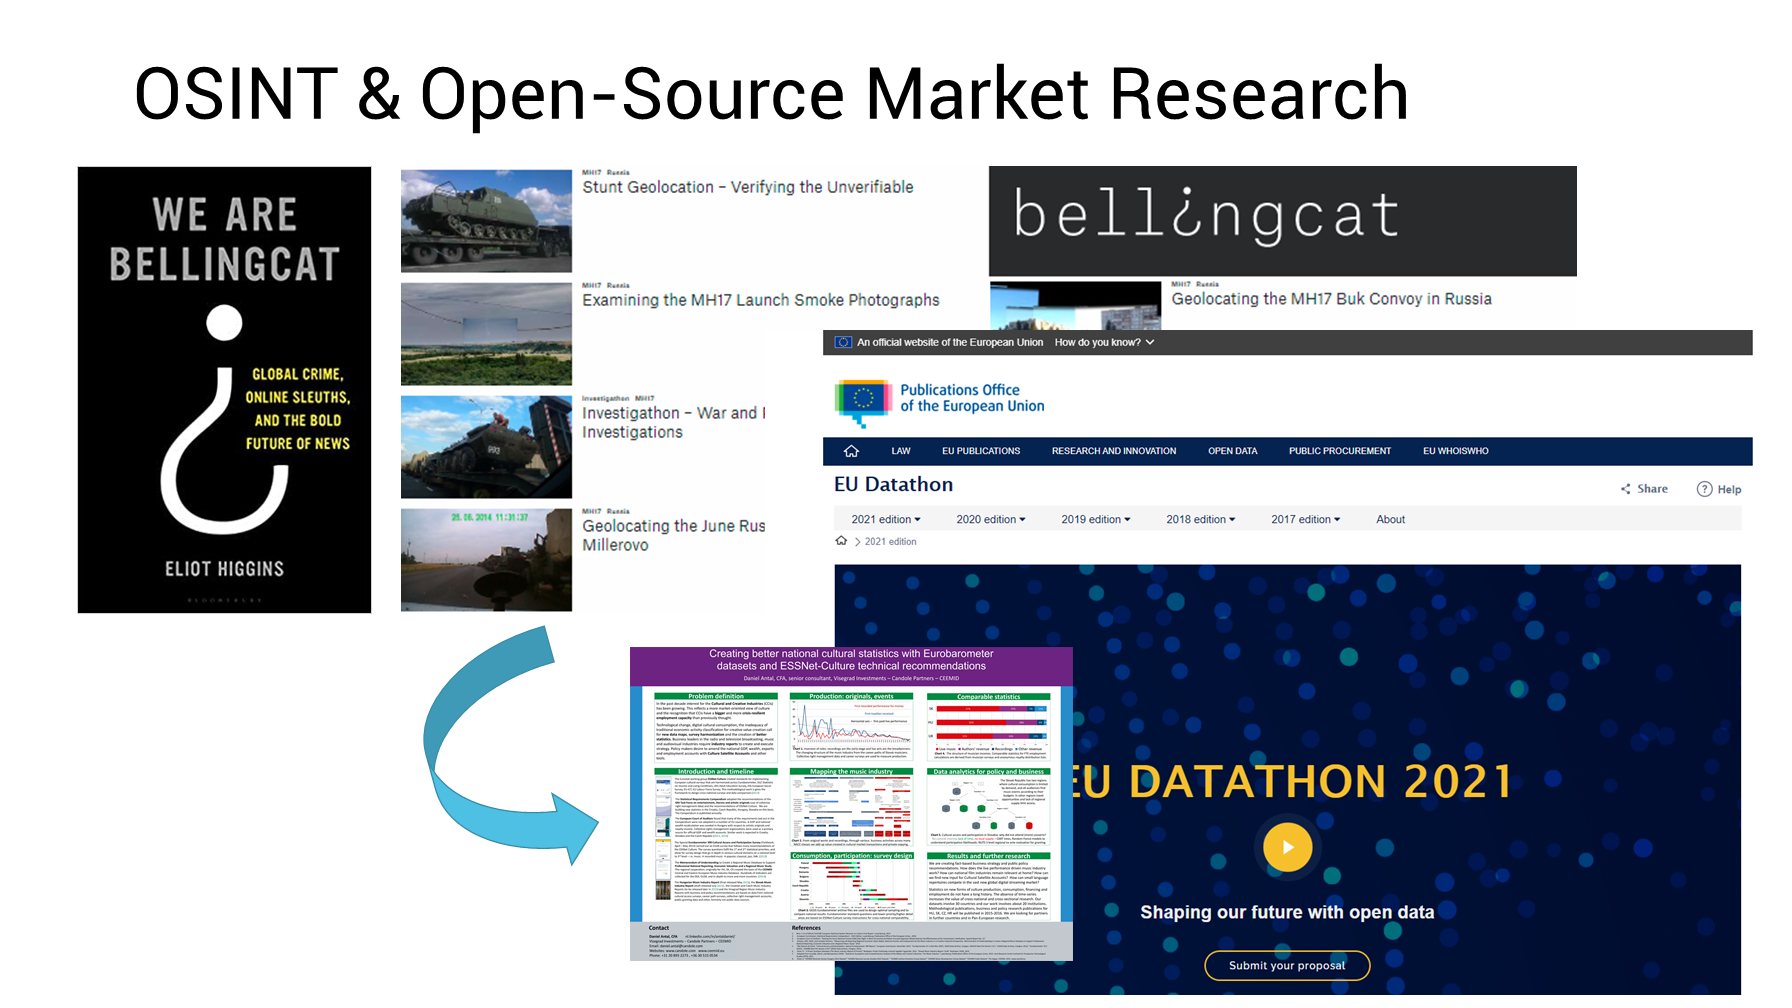
\includegraphics[width=24.89in]{C:/_bookdown/observatory_data_curators/plots/slides/open_source_slide} \end{center}

\hypertarget{add-value}{%
\section{How We Add Value to Data}\label{add-value}}

While the EU announces every year that again billions and billions of worth data became ``open'' again, this is not gold. At least not in the form of nicely minted gold coins, but in gold dust and nuggets found in the muddy banks of chilly rivers. There is no rush for it, because panning out its value requires plenty of hard work. We are trying to automate this work to make open data useable at scale, even in trustworthy AI solutions.

\begin{center}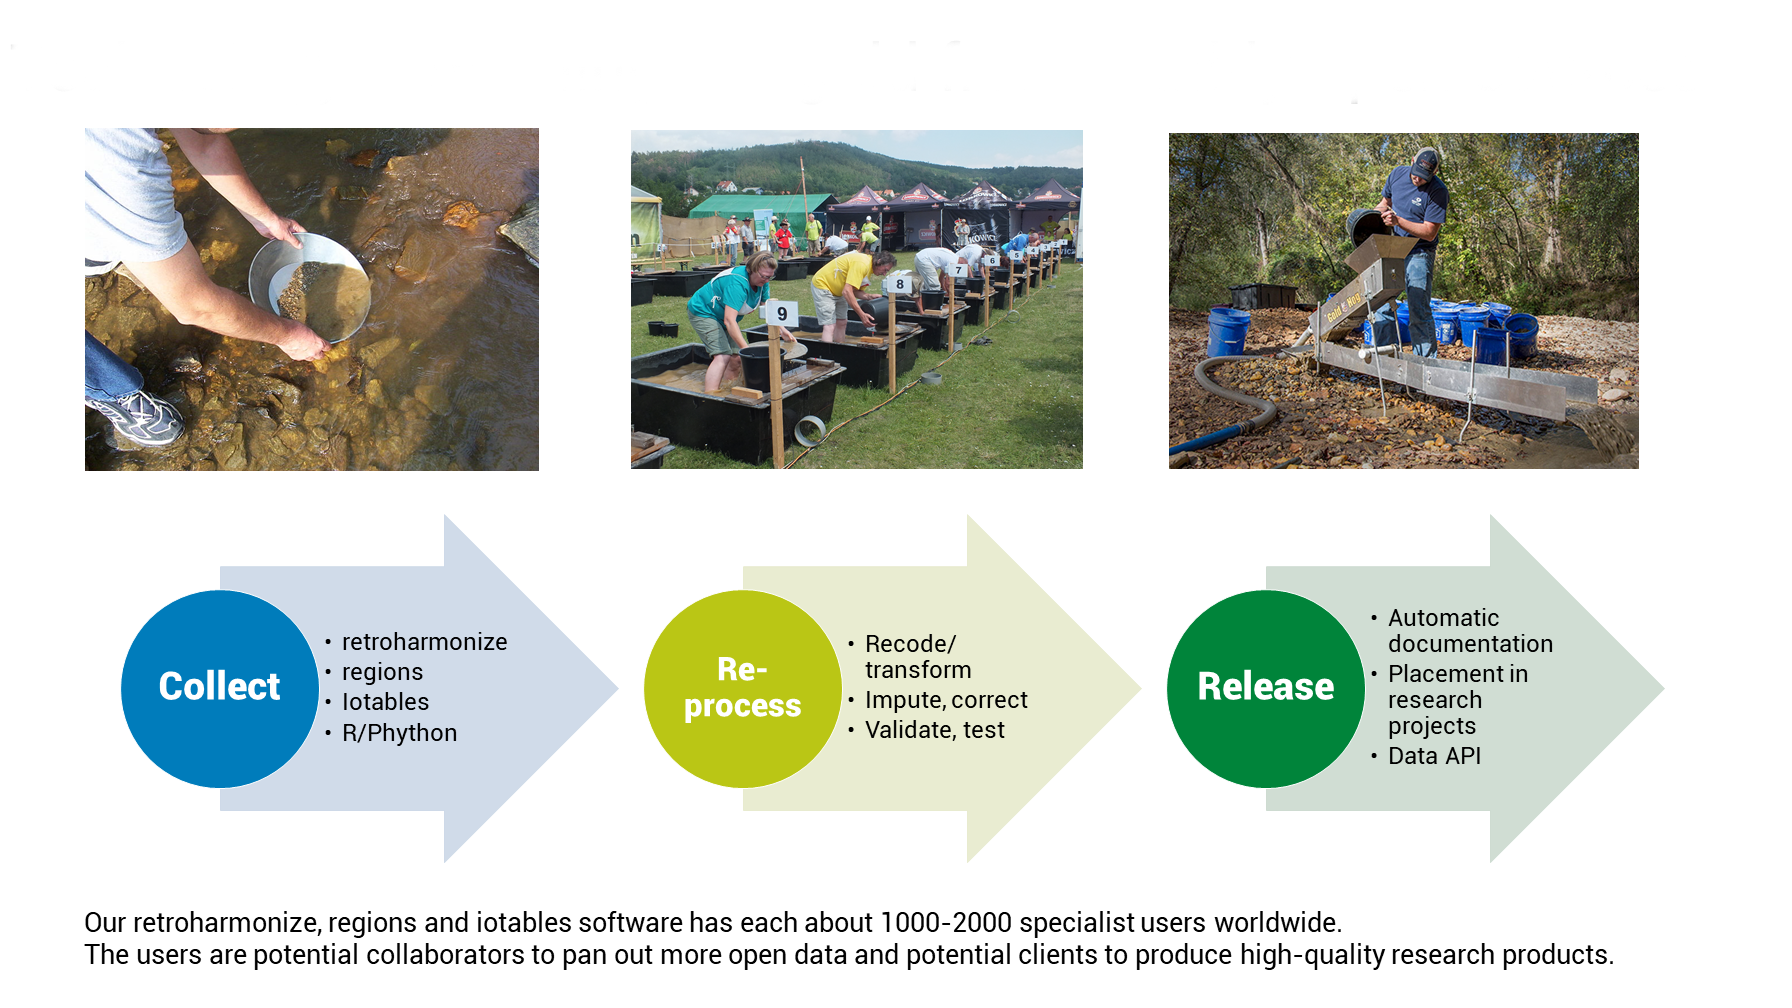
\includegraphics[width=24.89in]{C:/_bookdown/observatory_data_curators/plots/slides/gold_panning_slide_notitle} \end{center}

Most open data is not public, it is not downloadable from the Internet -- in the EU parlance, ``open'' only means a legal entitlement to get access to it. And even in the rare cases when data is open and public, often it is mired by data quality issues. We are working on the prototypes of a data-as-serve and research-as-service built with open-source statistical software that taps into various and often neglected open data sources.

We are in a prototype phase in June, but we hope that we will have a well-functioning service by the time of the conference, because we are working only with open-source software elements; our technological readiness level is already very high. The novelty of our process is that we are trying to further develop and integrate a few open-source technology items into a technologically and financially sustainable data-as-service and even research-as-service solutions.

We decided to take a new, modern approach to the `data observatory' concept, and modernize it with the application of 21st century data and metadata standards, the new results of reproducible research and data science. See \ref{service}. \protect\hyperlink{service}{Service Design and Business Case Development}

\hypertarget{reproducible-research}{%
\section{Reproducible Research}\label{reproducible-research}}

\begin{enumerate}
\def\labelenumi{\arabic{enumi}.}
\item
  \textbf{Our curatotrs} help finding the best available information source. This is often open data, which is not equal to public data. Open data is a governmental or scientific data source which you can legally access. It is almost never available for direct download, and requires much processing. You could probably do this in Excel -- if the data was not in various \texttt{sql}, \texttt{pdf}, \texttt{sav}, \texttt{csv}, \texttt{tsv}, \texttt{xls} and various other file formats.
\item
  \textbf{We process the data}: Yes, anybody can convert from millions of euros to euros in a spreadsheet, tons to kilograms, maybe even ounces to grams, but many unit conversions are error-prone if done by humans. Not everybody can make valid currency translations (\emph{When do I use year-end USD/EUR rate? Today's EUR/GBP? Or GBP/EUR? Annual average rate?}) We do this processing in a way that conforms to the tidy data definition, which allows easy integration, joining, and importing of data into your database. While the unit conversions can be automated in Excel or PowerBI, the data tidying requires a more programatic approach.
\item
  \textbf{Quality control}: Our data goes through dozens of computer logical checks (\emph{Do assets and liabilities match? Do dollar and euro amounts lead to the same result?}) Our algorithms go through automated and human statistical peer-review, and are open to your experts for checking, because transparency and openness allow for the best quality control. This unit testing is not really possible in Excel or Power BI, not to mention the senior supervision of such tasks. To maintain data integrity, we place an authoritative copy with a digital object identifier in the Zenodo scientific data repository. We place both our algorithms and our methods into peer-reviewed scientific publications, and our data products are checked and improved by competent experts in the field.
\item
  \textbf{We produce} the data and its visualization in easy to reuse, machine-readable, platform-independent formats. Just like that, \texttt{csv}, \texttt{json}, \texttt{jpg}, \texttt{png}, \texttt{doxc}, \texttt{epub}, \texttt{pdf}, \texttt{pptx}, \texttt{odt}, \texttt{sav}, you name it, we do it.
\end{enumerate}

\textbf{Reproducible research} is a scientific concept that can be applied to a wide range of professional designations, such as accounting, finance or the legal profession. We are applying this concept to \protect\hyperlink{opa}{Evidence-based, Open Policy Analysis} and \protect\hyperlink{business-professional-standards}{Professional Standards in Business}, including, for example, reproducible finance in the investment process or reproducible impact assessment in policy consulting. Based on computational reproducibility we believe that the following principles should be followed:
- \textbf{Reviewability} means that our application's results are can be assessed and judged by our user's experts, or experts they trust.
- \textbf{Reproducibility} means that we provide data products and tools that allow the exact duplication of our results during assessments. This ensures that all logical steps can be verified.
- \textbf{Confirmability} means that using our applications findings leads to the same professional results as other available software and information. Our data products use the open-source statistical programming language R. We provide details about our algorithms and methodology to confirm our results in SPSS or Stata or sometimes even in Excel.
- \textbf{Auditability} means that our data and software is archived in a way that external auditors can later review, reproduce and confirm our findings. This is a \emph{stricter form of data retention} than most organizations apply, because we do not only archive results step-by-step but all computational steps -- as if your colleagues would not only save every step in Excel but also their keystrokes. \protect\hyperlink{reproducible-research-theory}{Read more about this topic here}.

\begin{center}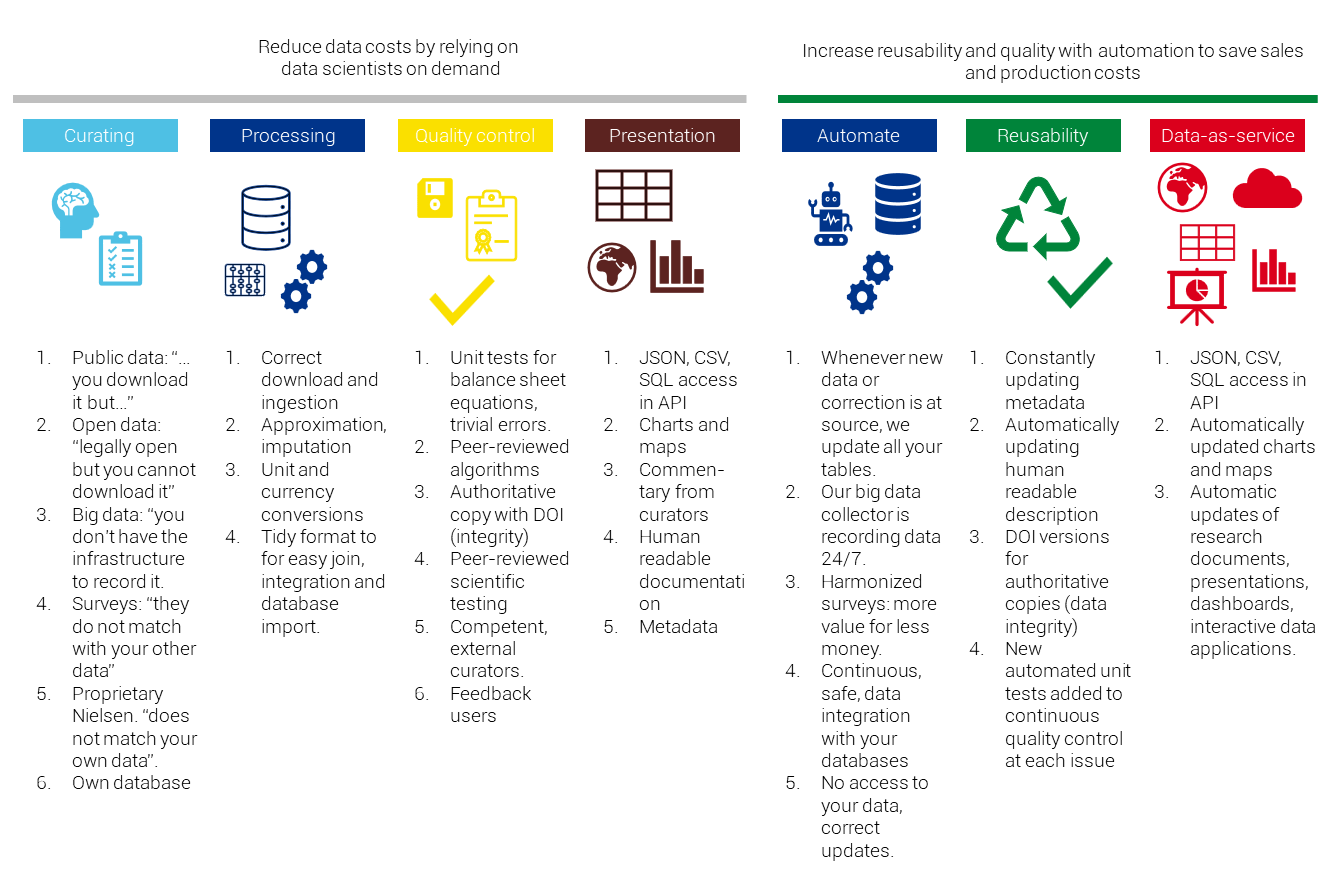
\includegraphics[width=18.67in]{plots/business_development/value_chain} \end{center}

\hypertarget{reproducible-research-theory}{%
\subsection{Reproducible Research}\label{reproducible-research-theory}}

\textbf{Reproducible research} is a scientific concept that can be applied to a wide range of professional designations. We are applying this concept to \protect\hyperlink{opa}{Evidence-based, Open Policy Analysis} and \protect\hyperlink{business-professional-standards}{Professional Standards in Business},
for example, reproducible finance in the investment process or reproducible impact assessment in policy consulting. Based on the computational reproducibility we believe that the following principles should be followed.

\begin{itemize}
\item
  \textbf{Reviewability} means that our application's results are can be assessed and judged by our user's experts, or experts they trust. We help reviewability with full transparency: we publish the software code that created the indicators, our methodology, and an automatically refreshing statistical description of the indicator each day when it receives new data or corrections from the original source.
\item
  \textbf{Reproducibility} means that we are providing data products and tools that allow the exact duplication of our results during assessments. This ensures that all logical steps can be verified. Reproducibility ensures that there is no lock-in to our applications. You can always chose a different data and software vendor, or compare our results with them.
\item
  \textbf{Confirmability} means that using our applications findings leads to the same professional results as other available software and information. Our data products use the open-source statistical programming language R. We provide details about our algorithms and methodology to confirm our results in SPSS or Stata or sometimes even in Excel.
\item
  \textbf{Auditability} means that our data and software is archived in a way that external auditors can later review, reproduce and confirm our findings. This is a \emph{stricter form of data retention} that most organizations apply, because we do not only archive results step-by-step but all computational steps -- as if your colleagues would not only save every step in Excel but also their keystrokes. While auditability is a requirement in accounting, we are extending this approach to all the quantitative work of a professional organization in an advisory or consulting capacity.
\item
  \textbf{Reviewable findings}: The descriptions of the methods can be independently assessed, and the results judged credible. In our view, this is a fundamental requirement for all professional applications. CEEMID's music data is used to settle royalty disputes in judicial procedures, or in grant and policy design. We believe that the future European Music Observatory should aim at the same bar, making its data \& research products open for challenges in the publicity of science, courts, and professional peers.
\item
  \textbf{Replicable findings}: We are presenting our findings and provide tools so that our users or auditors or external authorities can duplicate our results.
\item
  \textbf{Confirmable findings}: The main conclusions of the research can be obtained independently without our software, because we describe in detail the algorithms and methodology in supplementary materials. We believe that other organizations, analysts, statisticians must come to the same findings with their own methods and software. This avoids lock-in and allows independent cross-examination.
\item
  \textbf{Auditable findings}: Sufficient records (including data and software) have been archived so that the research can be defended later if necessary or differences between independent confirmations resolved. The archive might be private, as with traditional laboratory notebooks. See \protect\hyperlink{opencollaboration}{Open collaboration} with academia, auditors, and industry.
\end{itemize}

These computational requirements require a data workflow that relies on further principles.

\begin{itemize}
\item
  \textbf{Record retention}: all aspects of reproducibility require a high level of standardized documentation. The standardization of documentation requires the use of standardized metadata, metadata structures, taxonomies, vocabularies.
\item
  \textbf{Best available information / data universe}: the quality of the findings, their confirmation and auditing success will improve with better data and facts used.
\item
  \textbf{Data validations}: The quality of the findings will greatly depend on the factual inputs. While the reproducible findings may have many problems, inputting erroneous data or faulty information will likely lead to wrong conclusions, and in all cases will make confirmation and auditing impossible. Especially when organizations use large and heterogeneous data sources, even small errors, such as erroneous currency translations or accidental misuse of decimals, units can cause results that will not pass confirmation or auditing.
\end{itemize}

\hypertarget{fair}{%
\section{FAIR}\label{fair}}

In 2016, the `\textbf{\href{http://www.nature.com/articles/sdata201618}{FAIR Guiding Principles for scientific data management and stewardship'}} were published in \emph{Scientific Data}. The authors intended to provide guidelines to improve the \textbf{F}indability, \textbf{A}ccessibility, \textbf{I}nteroperability, and \textbf{R}euse of digital assets. The principles emphasise machine-actionability (i.e., the capacity of computational systems to find, access, interoperate, and reuse data with none or minimal human intervention) because humans increasingly rely on computational support to deal with data as a result of the increase in volume, complexity, and creation speed of data.

We are trying to make our API service FAIR by automatically adding to our data standardized metadata that fulfills the mandatory requirements of the Dublic Core metadata standards and at the same time the \href{https://support.datacite.org/docs/datacite-metadata-schema-v44-mandatory-properties}{mandatory requirements}, and most of the \href{https://support.datacite.org/docs/datacite-metadata-schema-v44-recommended-and-optional-properties}{recommended requirements} of DataCite.

A practical ``how to'' guidance to go FAIR can be found in the \textbf{\href{https://www.go-fair.org/how-to-go-fair/}{Three-point FAIRification Framework}}.

\textbf{{F}indable}

The first step in (re)using data is to find them. Metadata and data should be easy to find for both humans and computers. Machine-readable metadata are essential for automatic discovery of datasets and services, so this is an essential component of the \textbf{\href{https://www.go-fair.org/fair-principles/fairification-process/}{FAIRification process}}.

\textbf{\href{https://www.go-fair.org/fair-principles/fair-data-principles-explained/f1-meta-data-assigned-globally-unique-persistent-identifiers/}{F1. (Meta)data are assigned a globally unique and persistent identifier}}

\textbf{\href{https://www.go-fair.org/fair-principles/fair-data-principles-explained/f2-data-described-rich-metadata/}{F2. Data are described with rich metadata (defined by R1 below)}}

\textbf{\href{https://www.go-fair.org/fair-principles/f3-metadata-clearly-explicitly-include-identifier-data-describe/}{F3. Metadata clearly and explicitly include the identifier of the data they describe}}

\textbf{\href{https://www.go-fair.org/fair-principles/f4-metadata-registered-indexed-searchable-resource/}{F4. (Meta)data are registered or indexed in a searchable resource}}

\textbf{{A}ccessible}

Once the user finds the required data, she/he/they need to know how can they be accessed, possibly including authentication and authorisation.

\textbf{\href{https://www.go-fair.org/fair-principles/542-2/}{A1. (Meta)data are retrievable by their identifier using a standardised communications protocol}}

\textbf{\href{https://www.go-fair.org/fair-principles/a1-1-protocol-open-free-universally-implementable/}{A1.1 The protocol is open, free, and universally implementable}}

\textbf{\href{https://www.go-fair.org/fair-principles/a1-2-protocol-allows-authentication-authorisation-required/}{A1.2 The protocol allows for an authentication and authorisation procedure, where necessary}}

\textbf{\href{https://www.go-fair.org/fair-principles/a2-metadata-accessible-even-data-no-longer-available/}{A2. Metadata are accessible, even when the data are no longer available}}

\textbf{{I}nteroperable}

The data usually need to be integrated with other data. In addition, the data need to interoperate with applications or workflows for analysis, storage, and processing.

\textbf{\href{https://www.go-fair.org/fair-principles/i1-metadata-use-formal-accessible-shared-broadly-applicable-language-knowledge-representation/}{I1. (Meta)data use a formal, accessible, shared, and broadly applicable language for knowledge representation.}}

\textbf{\href{https://www.go-fair.org/fair-principles/i2-metadata-use-vocabularies-follow-fair-principles/}{I2. (Meta)data use vocabularies that follow FAIR principles}}

\textbf{\href{https://www.go-fair.org/fair-principles/i3-metadata-include-qualified-references-metadata/}{I3. (Meta)data include qualified references to other (meta)data}}

\textbf{{R}eusable}

The ultimate goal of FAIR is to optimise the reuse of data. To achieve this, metadata and data should be well-described so that they can be replicated and/or combined in different settings.

\textbf{\href{https://www.go-fair.org/fair-principles/r1-metadata-richly-described-plurality-accurate-relevant-attributes/}{R1. (Meta)data are richly described with a plurality of accurate and relevant attributes}}

\textbf{\href{https://www.go-fair.org/fair-principles/r1-1-metadata-released-clear-accessible-data-usage-license/}{R1.1. (Meta)data are released with a clear and accessible data usage license}}

\textbf{\href{https://www.go-fair.org/fair-principles/r1-2-metadata-associated-detailed-provenance/}{R1.2. (Meta)data are associated with detailed provenance}}

\textbf{\href{https://www.go-fair.org/fair-principles/r1-3-metadata-meet-domain-relevant-community-standards/}{R1.3. (Meta)data meet domain-relevant community standards}}

The principles refer to three types of entities: data (or any digital object), metadata (information about that digital object), and infrastructure. For instance, principle F4 defines that both metadata and data are registered or indexed in a searchable resource (the infrastructure component).

\hypertarget{app}{%
\chapter{Application: Automated Data Observatories}\label{app}}

This year's EU Datathlon includes three challenges. We are contesting all three of them with the same technology and knowledge management, but with different data used in a wide range of knowledge domains.

\hypertarget{data-acquisition-and-processing}{%
\section{Data Acquisition and Processing}\label{data-acquisition-and-processing}}

We access various open governmental and open scientific sources programatically. Our programs are mainly written in the R language, but we have a growing body of software written in Python, too. We thrive to be open for both R and Python developers, and as much as possible, exploit the synergies between the more statistically oriented R language and the more genereal application-oriented Python. We welcome \href{https://economy.dataobservatory.eu/authors/curator/}{curators} and \href{https://greendeal.dataobservatory.eu/authors/developer/}{developers} in both languages.

An important aspect of our quality control is that our processing code is open and peer-reviewed. Our observatories are turning the peer-reviewed statistical software of the \href{http://ropengov.org/}{rOpenGov} community into a continous data-as-service product. This means that we are creating collector software that is making reproducible data assets, mainly business and policy indicators. Then we are running this software daily in the cloud, and place the new data acquisitions' \protect\hyperlink{zenodo}{authoritative copies} into a scientific repository for data integrity purposes, then upload it to our \protect\hyperlink{api}{API}, describe it in our \protect\hyperlink{bookdown}{long form documentation}, and eventually blog about the newsworthy finds on our \protect\hyperlink{hugo}{Front-end Websites}.

The entire research automation system is maintained by \href{https://reprex.nl/}{Reprex}, a Dutch research automation startup, in open collaboration with \href{http://ropengov.org/}{rOpenGov} and other \href{https://greendeal.dataobservatory.eu/\#contributors}{developers}.

\hypertarget{zenodo}{%
\section{Data Integrity: Authoritative Copies}\label{zenodo}}

We rely on a data repository to keep a final, authoritative copy of our data assets and visualizations. This repository is independent from us.

Zenodo is a semi-endorsed EU solution, originating from CERN. In the last EU budget period all EU-funded research was supposed to deposit data there, although this requirement was not often enforced. Manual deposition is in working order, and we can very easily retrieve our own data in various versions. It is also free data storage.

The Zenodo API is not very well documented, particularly for R. But it is supported both in Python and R. We have a tutorial and code on how to deposit our assets programatically via the \href{https://github.com/eblondel/zen4R/wiki}{Zen4R} package. It is a bit difficult to use - it mimics ``true'' object oriented programming relying on R6 classes, which is extremely rarely used by R programmers.

The Dataverse is much better served, the API is better documented, and technically we could even set up our own instance (new dataverses can be installed.) The best instance is of course the original Harvard Dataverse. Currently Dataverse has no support on CRAN - the R package was just kicked out of CRAN, and it is buggy, but it can be fixed. Should there be a need, we can make a connector to Dataverse, too.

\hypertarget{api}{%
\section{Automated Data Observatory API}\label{api}}

Our observatories APIs are \href{https://datasette.io/}{Datasette} instances. It is a lightweight, Python-based application that turns a SQLite database into a powerful API. Our developer, \href{https://music.dataobservatory.eu/author/botond-vitos/}{Botond Vitos} manages our APIs.

The indicator table contains the actual values, and the various estimated/imputed values of the indicator, clearly marking missing values, too.

\begin{center}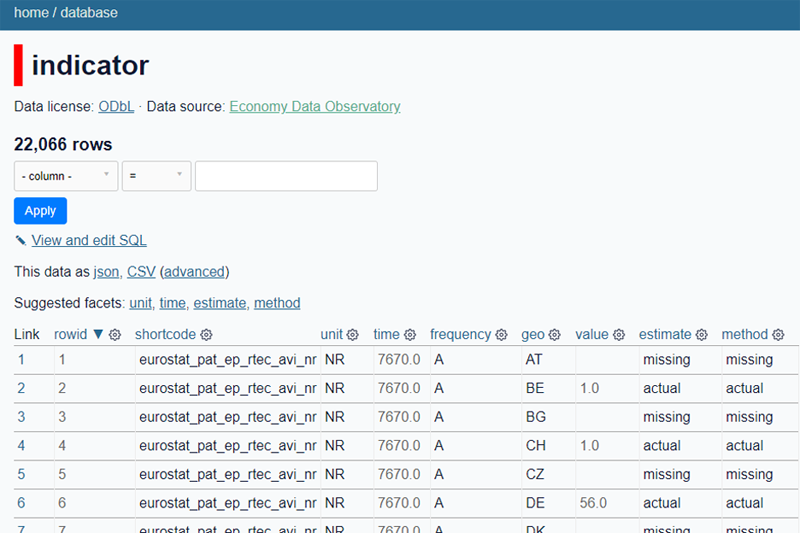
\includegraphics[width=11.11in]{plots/screenshots/EDO_API_indicator_table} \end{center}

The descriptive metadata is contained in the \textbf{description} tables.

\begin{center}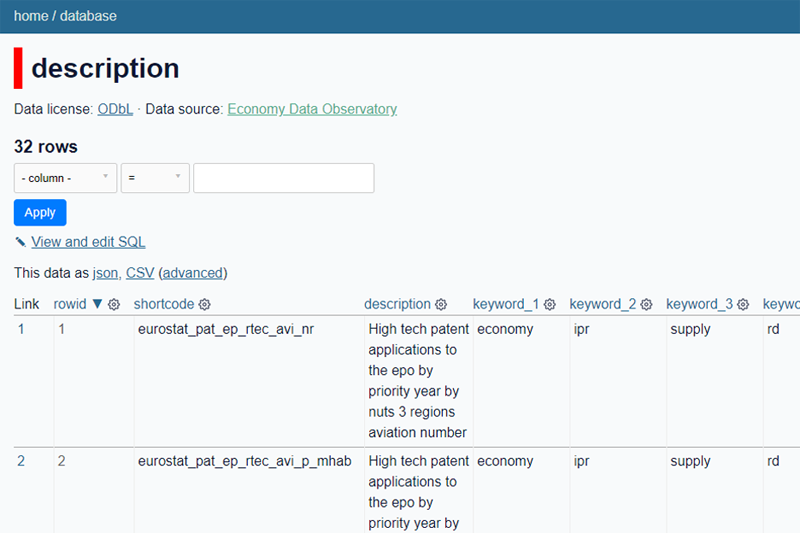
\includegraphics[width=11.11in]{plots/screenshots/EDO_API_description_table} \end{center}

The data transactional and processing metadata is contained in the \textbf{metadata} tables.

\begin{center}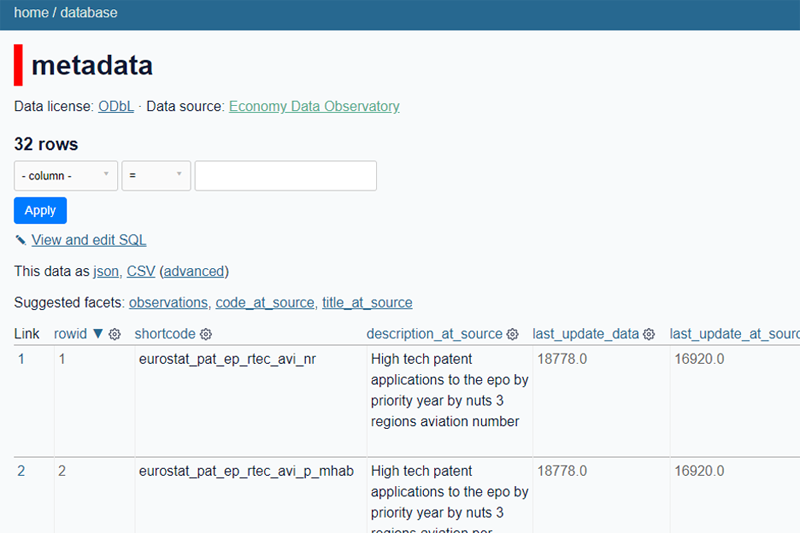
\includegraphics[width=11.11in]{plots/screenshots/EDO_API_metadata_table} \end{center}

The variable labelling and unit labelling information is stored in the \textbf{labelling} tables.

\begin{center}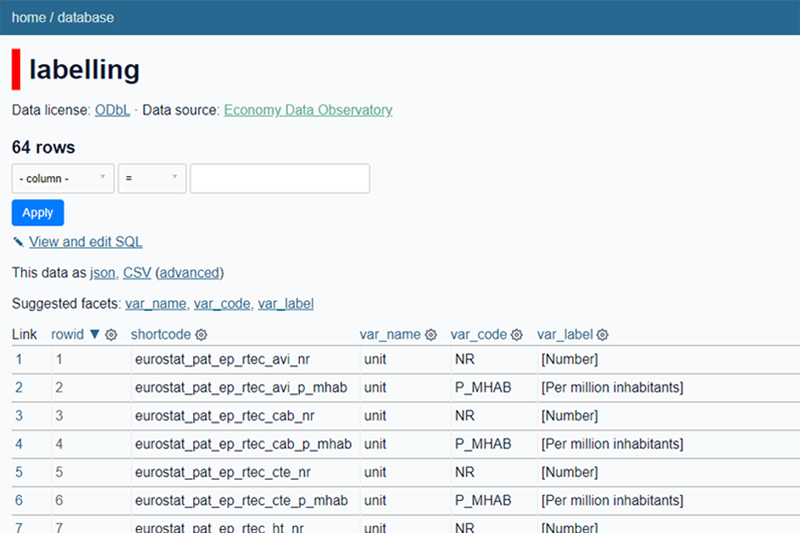
\includegraphics[width=11.11in]{plots/screenshots/EDO_API_labelling_table} \end{center}

Currently our APIs are re-freshed by an R code. We will soon add a Python collector, too.

\hypertarget{bookdown}{%
\section{Long form documentation}\label{bookdown}}

Our long-form documentation is based on \href{https://bookdown.org/yihui/bookdown/}{bookdown}, which relies on pandoc, rmarkdown and knitr. This handbook is also created in bookdown.

\begin{center}
\includegraphics[width=5.89in]{plots/bookdown} \end{center}

It is a very mature workflow, it produces a long-form website, and PDF, ePUB or Word versions from the API. The current automation is not operational, as we have recently included the API.

\hypertarget{hugo}{%
\section{Front-End Websites}\label{hugo}}

Our observatory's client-facing front end is made by the static website generator hugo, which is programmed in the \texttt{go} language. We use the open-source \href{https://github.com/wowchemy/starter-hugo-academic}{Starter Hugo Academic} template of \href{https://wowchemy.com/docs/getting-started/page-builder/}{wowchemy}. If we win a price, we'll certainly offer them a share!

\begin{center}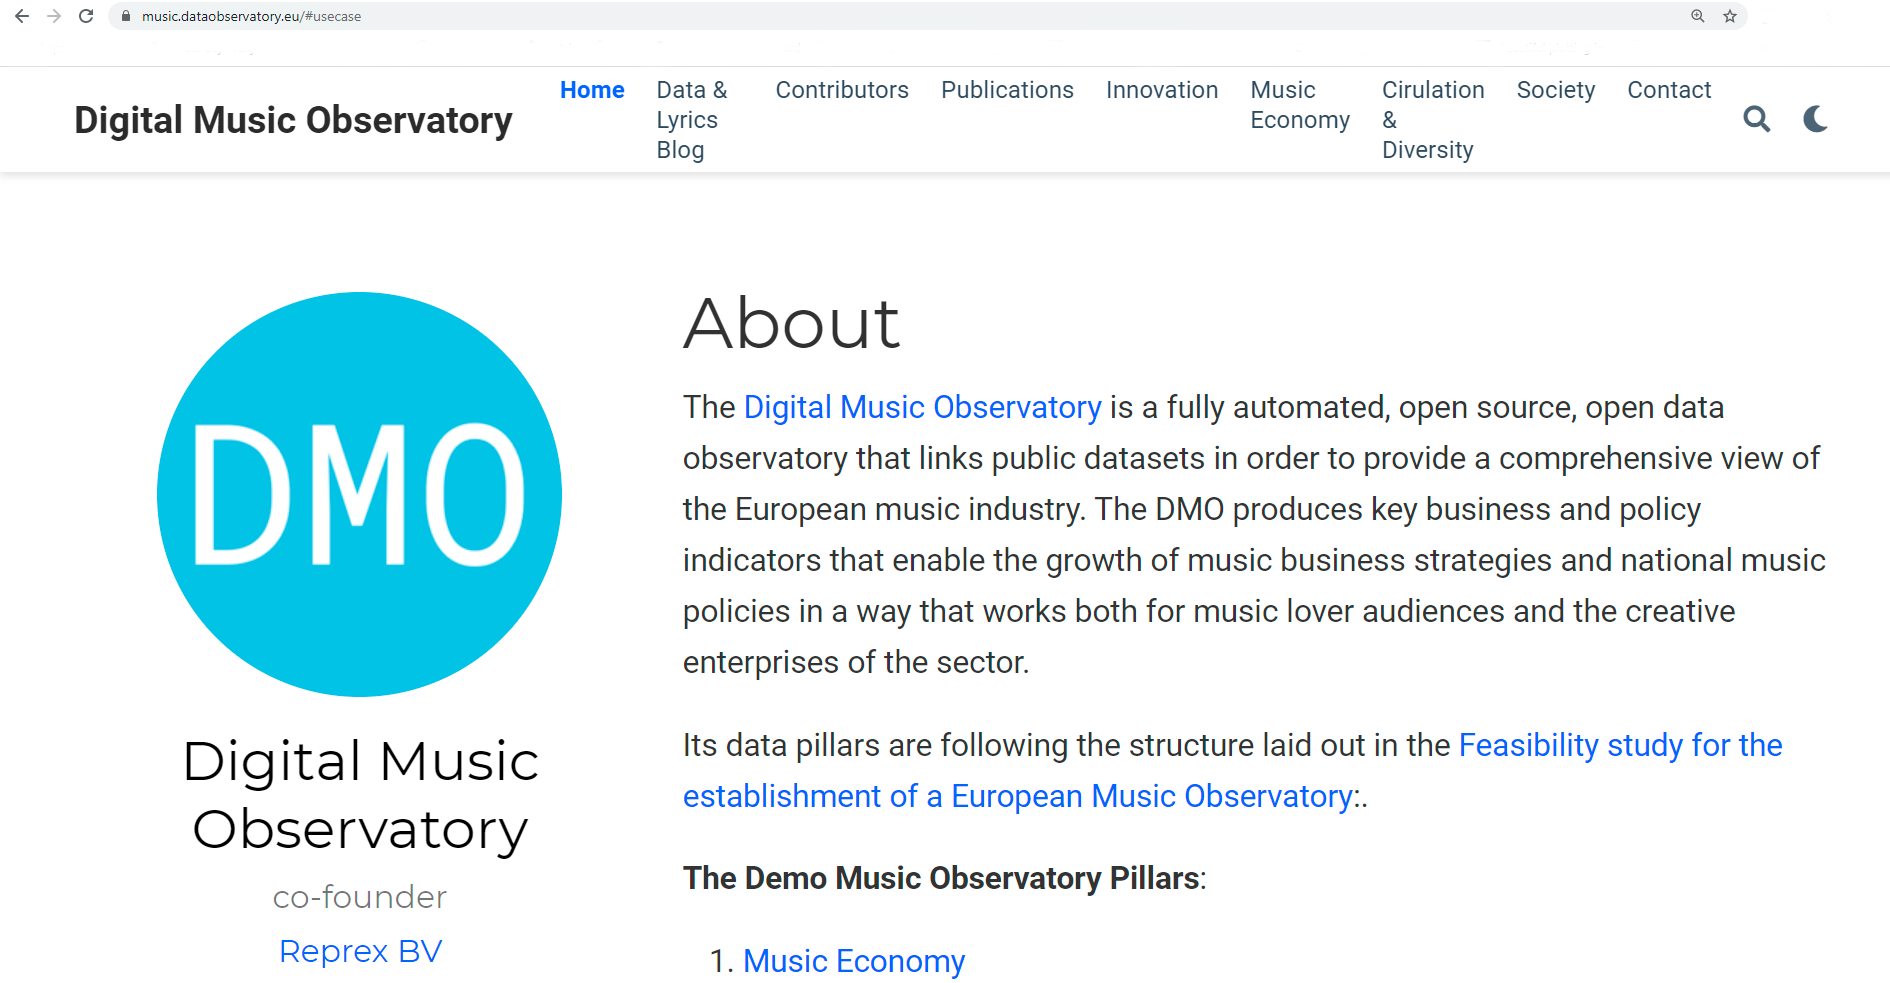
\includegraphics[width=26.25in]{plots/screenshots/dmo_opening_screen} \end{center}

The hugo-bookdown integration is partly supported by the R package \href{https://bookdown.org/yihui/blogdown/}{blogdown}. This is a semi-success, and while academic is a super-popular template, it is getting further and further away from blogdown. The original advantage is that it can be managed in the same workflow as the indicator generation, package documentation, the long-form documentation is a bit gone.

\begin{center}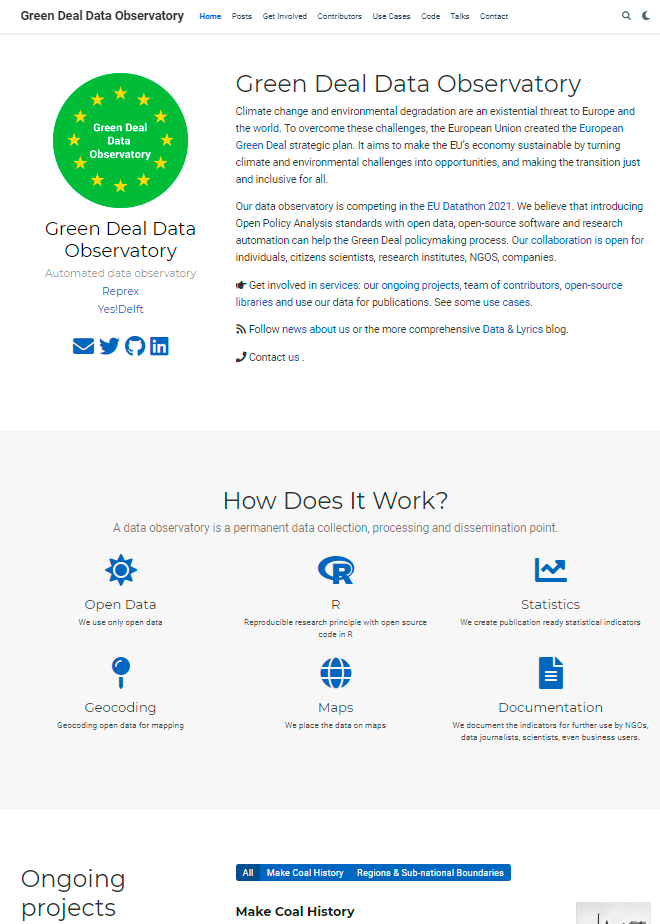
\includegraphics[width=9.17in]{plots/green_deal_hugo} \end{center}

\hypertarget{research-automation}{%
\section{Research Automation}\label{research-automation}}

Because every step of our data acquisition, processing, structuring, and testing is going through machines, it can be replicated any given year, month, day, or hour. Research automation means that we update our data every day (Is there new data at the source? Corrections? Known issues?) and place the current version in an API.

\begin{enumerate}
\def\labelenumi{\arabic{enumi}.}
\item
  \textbf{Continous data collection}: Big data sources usually provide the user with a large quantity of insignificant data. Because of the large quantity, the data is usually not available historically: you capture it today or it is gone. You need to process data in big quantities in order to find signficiant and meaningful information. Most small enterprises and research teams do not have the engineering capactity to organize this. We do continous data collection on all sources to capture the latest updates, or corrections.
\item
  \textbf{Focus on reusability}: In our experience, the resuability of research and consulting work is greatly reduced by two factors, which we resolve with continous data collection and documentation:

  \begin{itemize}
  \tightlist
  \item
    poor documentation (the bibliography updates and file descriptions are the least priortized tasks)
  \item
    data tables, charts, visualizations became dated then obsolete.
  \end{itemize}
\item
  From tidy and open data to \textbf{data-as-service}: Because all our assets, including key business indicators, policy indicators, scientific replication sets, and their visualizations, as well as maps, are created by open source and reproducible software, the software can run continously. Instead of providing our users with data tables, charts and maps, we provide them with a subsription to the latest data and its latest visualizations.
\end{enumerate}

\hypertarget{service}{%
\chapter{Service Design and Business Case Development}\label{service}}

We decided to take a new, modern approach to the `data observatory' concept, and modernize it with the application of 21st century data and metadata standards, the new results of reproducible research and data science. Various UN and OECD bodies, and particularly the European Union support or maintain more than 60 data observatories, or permanent data collection and dissemination points, but even these do not use these organizations and their members open data.

We are building open-source data observatories, which run open-source statistical software that automatically processes and documents reusable public sector data (from public transport, meteorology, tax offices, taxpayer funded satellite systems, etc.) and reusable scientific data (from EU taxpayer funded research) into new, high quality statistical indicators.

We are building various open-source data collection tools in R and Python to bring up data from big data APIs and legally open, but not public, and not well served data sources. For example, we are working on capturing representative data from the Spotify API or creating harmonized datasets from the Eurobarometer and Afrobarometer survey programs.

Open data is usually not public; whatever is legally accessible is usually not ready to use for commercial or scientific purposes. In Europe, almost all taxpayer funded data is legally open for reuse, but it is usually stored in heterogenous formats, processed into an original government or scientific need, and with various and low documentation standards. Our expert data curators are looking for new data sources that should be (re-) processed and re-documented to be usable for a wider community.

We would like to introduce our service flow, which touches upon many important aspects of data scientist, data engineer and data curatorial work.

\begin{itemize}
\tightlist
\item
  We believe that even such generally trusted data sources as Eurostat often need to be reprocessed, because various legal and political constraints do not allow the common European statistical services to provide optimal quality data -- for example, on the regional and city levels.
\item
  With rOpenGov and other partners we are creating open-source statistical software in R to re-process these heterogenous and low-quality data into tidy statistical indicators, and automatically validate, and document it.
\item
  We are carefully documenting and releasing administrative, processing, and descriptive metadata, following international metadata standards, to make our data easy to find and easy to use for data analysist.
\item
  We are automatically creating depositions and authoritative copies marked with an individual digital object identifier (DOI) to maintain data integrity.
\item
  We are building a simple database and supporting API that releases the data without restrictions, in a tidy format that is easy to join with other data, or easy to join into databases, together with standardized metadata.
\item
  We maintain observatory website where not only the data is available, but we are placing tutorials and use cases to make it easier to use them. Our aim is to show a modern, 21st century reimagination of the data observatory concept developed and supported by the UN, EU and OECD, and we want to show that modern reproducible research and open data could make the existing 60 data observatories and the planned new ones grow faster into data ecosystems.
\end{itemize}

We are working around the open collaboration concept, which is well-known in open source software development and reproducible science, but we try to make this agile project management methodology more inclusive, and include data curators, and various institutional partners into this approach. Based around our early-stage startup, Reprex, and the open-source developer community rOpenGov, we are working together with other developers, data scientists, and domain specific data experts in climate change and mitigation, antitrust and innovation policies, and various aspect of the music and film industry.

\begin{figure}

{\centering 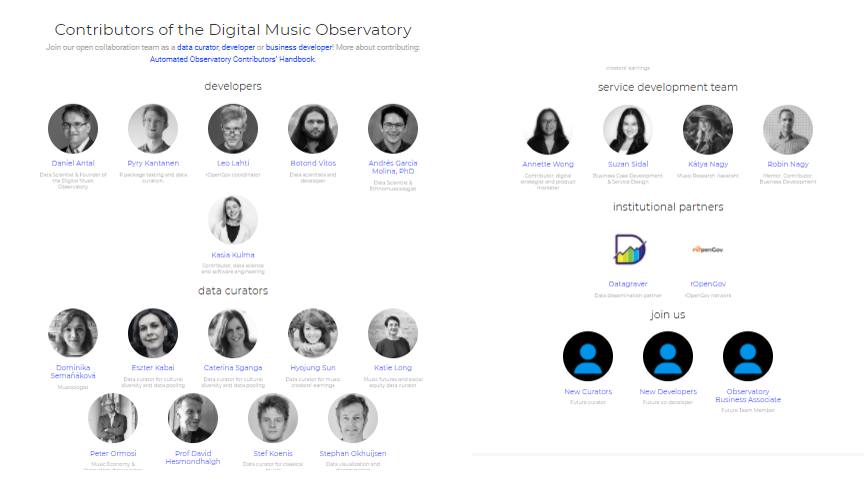
\includegraphics[width=12.06in]{C:/_bookdown/observatory_data_curators/plots/screenshots/dmo_contributors} 

}

\caption{Our open collaboration is truly open: new data curators, data scientists and data engineers are welcome to join in.}\label{fig:unnamed-chunk-2}
\end{figure}

Our open collaboration is truly open: new data curators, data scientists and data engineers are welcome to join in. We develop open-source software in an agile way, so you can join in with an intermediate programming skill to build unit tests or add new functionality, and if you are beginner, you can start with documentation and testing our tutorials. For business, policy, and scientific data analysts, we provide unexploited, exciting new datasets. And of course, advanced developers can join our development team: the statistical data creation is mainly made in the R language, and the service infrastructure in Python and Go components.

\hypertarget{business-professional-standards}{%
\section{Professional Standards in Business}\label{business-professional-standards}}

\hypertarget{key-business-indicators}{%
\subsection{Key Business Indicators}\label{key-business-indicators}}

\hypertarget{business-record-retention}{%
\subsection{Business Record Retention}\label{business-record-retention}}

Some of the requirements of reproducible research are usually required by professional standards. For example, various accounting, finance, legal or consulting professional standards call for appropriate documentation and record retention.

\hypertarget{policy-professional-standards}{%
\section{Professional Standards in Policy}\label{policy-professional-standards}}

\hypertarget{opa}{%
\subsection{Evidence-based, Open Policy Analysis}\label{opa}}

In the last two decades, governments and researchers have placed a growing emphasis on the value of evidence-based policy. However, while the evidence generated through research to inform policy has become more rigorous and transparent, policy analysis--the process of contextualizing evidence to inform specific policy decisions--remains opaque.

We believe that a modern data observatory must improve how evidence is created and used in policy reports, and pass on the efficiency gains from increasing reproducibility and automation. Therefore, we pledge that the \href{https://music.dataobservatory.eu}{music.dataobservatory.eu} will comply with the \href{https://www.bitss.org/opa/}{Open Policy Analysis} standards developed by the \href{https://www.bitss.org/}{Berkeley Initiative for Transparency in the Social Sciences} \& \href{https://cega.berkeley.edu/}{Center for Effective Global Action}. These standards are applied by the World Bank.

\hypertarget{contributors}{%
\section{Contributors}\label{contributors}}

We are looking for business associates to help our service design into our

\begin{itemize}
\item
  \href{https://greendeal.dataobservatory.eu/\#contributors}{Green Deal Data Observatory}
\item
  \href{https://economy.dataobservatory.eu/\#contributors}{Economy Data Observatory}
\item
  \href{https://music.dataobservatory.eu/\#contributors}{Digital Music Observatory}
\end{itemize}

\begin{enumerate}
\def\labelenumi{\arabic{enumi}.}
\item
  Work with governmental or scientific or otherwise \protect\hyperlink{open-data}{open data}.
\item
  Committed to high policy or business professional standards, and by making their work \protect\hyperlink{reproducible-research}{reproducible}, they adhere to reviewability, reproducability, confirmability and auditability, regardless if they work, or study for various professsional roles in business, academia, public or non-governmental policy, and data journalism.
\end{enumerate}

\begin{quote}
An important aspect of the EU Datathon Challenges is ``.. to propose the development of an application that links and uses open datasets {[}\ldots{]} to find suitable new approaches and solutions to help Europe achieve important goals set by the European Commission through the use of open data.''
\end{quote}

Where to find us:
- \href{https://github.com/dataobservatory-eu}{dataobservatory-eu} is our private repo collection and private github collaboration platform, but many of our repos are open. Like this one.

\begin{itemize}
\item
  \href{https://www.linkedin.com/company/reprexbv/}{Creative Data Observatories LinkedIn Page}. Make sure you follow us, and spread our messages.
\item
  \href{https://twitter.com/dataandlyrics}{twitter.com/dataandlyrics} is our twitter handle for our music-oriented blog. If you are on twitter, please follow us, and retweet our blogposts.
\item
  \href{https://keybase.io/team/reprexcommunity}{keybase.io/team/reprexcommunity} is our landing page to our otherwise private and invisible internal communication platform. (See more in subchapter\ref{keybase} of \protect\hyperlink{keybase}{Tools}.)
\end{itemize}

You find more information in the \ref{data-curators} chapter about our topics: \protect\hyperlink{open-data}{What is Open Data?}, \protect\hyperlink{reproducible-research-theory}{Reproducible Research}, and of course, \protect\hyperlink{get-inspired}{Get Inspired About Data}.

\hypertarget{topic-associate}{%
\section{Passion About Our Topic}\label{topic-associate}}

\begin{itemize}
\item
  You are passionate about one of our topics, but you do not feel that you have the skills yet to become a data curator or a developer.
\item
  You have a curiosity in the field of economic policies, particularly in computational antitrust, innovation research, and understanding the statistically under-represented micro- and small enterprises, join our \href{https://economy.dataobservatory.eu/\#contributors}{Economy Data Observatory} as a volunteer.
\item
  You are passionate about environmental research of climate change, designing urban, social and economic mitigation strategies, or undertanding how people think about climate change, join our \href{https://greendeal.dataobservatory.eu/\#contributors}{Green Deal Data Observatory} team as a volunteer.
\item
  You want to know how musicians can make a living after the pandemic? How can we make sure that music made by womxn, small country artists or artists of color gets and equal chance? Are you interested in the future of ethical AI and data governance? Join our \href{https://music.dataobservatory.eu/\#contributors}{Digital Music Observatory} team as a volunteer.
\end{itemize}

\hypertarget{open-associate}{%
\section{Passion For Trustworthy AI, Open Data and Open Source Projects}\label{open-associate}}

\begin{itemize}
\item
  You want to learn to write scientifically valid, open source code in R or Python, but you are a beginner. We help you anywhere - you can even start copyediting or technical documentation (it is a must in open source development) and create tutorials for you to interact with our data and products (if if helps you, it will help others.)
\item
  As a business economist or legal professional, you are interested how open data, open source software, research automation and ethical, trustworthy AI products can find their market.
\item
  As a blogger, data journalist or marketeer you would like to help to make open data, and transparent, ethical, open AI more widely known and used.
\end{itemize}

\hypertarget{technical-requirements-associate}{%
\section{Technical Requirements}\label{technical-requirements-associate}}

\begin{itemize}
\item
  Make sure that you read the \href{https://www.contributor-covenant.org/}{Contributors Covenant}. You must make this \href{https://www.contributor-covenant.org/version/2/0/code_of_conduct/}{pledge} to make participation in our community a harassment-free experience for everyone, regardless of age, body size, visible or invisible disability, ethnicity, sex characteristics, gender identity and expression, level of experience, education, socio-economic status, nationality, personal appearance, race, caste, color, religion, or sexual identity and orientation. Participating in our data observatories requires everybody to act and interact in ways that contribute to an open, welcoming, diverse, inclusive, and healthy community. It's better this way for you and for us!
\item
  Give users at least one social media account where they can get in touch with you (any of LinkedIn, Twitter, Academia, SSRN, Google Scholar, or even Facebook.)
\item
  Please, follow us on social media, it really helps us finding new users and showing that we are able to grow our ecosystem.

  \begin{itemize}
  \tightlist
  \item
    \href{https://www.linkedin.com/company/78556699}{Green Deal Data Observatory on Linkedin} and \href{https://twitter.com/GreenDealObs}{Green Deal Data Observatory on Twitter}
  \item
    \href{https://www.linkedin.com/company/78562153}{Economy Data Observatory on Linkedin} and \href{https://twitter.com/GreenDealObs}{Economy Data Observatory on Twitter}
  \item
    \href{https://www.linkedin.com/company/reprexbv/}{Digital Music Data Observatory on Linkedin} and \href{https://twitter.com/dataandlyrics}{Digital Music Data Observatory on Twitter}
  \end{itemize}
\item
  Please send us back this \href{https://greendeal.dataobservatory.eu/media/documents/bio_template.md}{md file} with your data. You can open it with any text editor, but Notepad, TextEdit, Vim and similar clean text editors are the best.
\item
  If you feel you need chatting on onboarding, contact us on \href{https://curators.dataobservatory.eu/tools.html\#keybase}{Keybase} - it's lightweight, discrete, encrypted, your mother, partner and friends are not there, it is free, open source, and can share/exchange files, too. Otherwise in email.
\end{itemize}

\hypertarget{data-curators}{%
\chapter{Data Curators}\label{data-curators}}

We are looking for data curators into our

\begin{itemize}
\item
  \href{https://greendeal.dataobservatory.eu/\#contributors}{Green Deal Data Observatory}
\item
  \href{https://economy.dataobservatory.eu/\#contributors}{Economy Data Observatory}
\item
  \href{https://music.dataobservatory.eu/\#contributors}{Digital Music Observatory}
\end{itemize}

\begin{enumerate}
\def\labelenumi{\arabic{enumi}.}
\item
  Work with governmental or scientific or otherwise \protect\hyperlink{open-data}{open data}.
\item
  Committed to high policy or business professional standards, and by making their work \protect\hyperlink{reproducible-research}{reproducible}, they adhere to reviewability, reproducability, confirmability and auditability, regardless if they work, or study for various professsional roles in business, academia, public or non-governmental policy, and data journalism.
\item
  They are interested in helping us with \protect\hyperlink{indicator-design}{indicator design}.
\item
  Make the authoritative copy of their indicator available on the Zenodo data repository, and keep it up-to-date with our automated observatory's help.
\end{enumerate}

\begin{quote}
An important aspect of the EU Datathon Challenges is ``.. to propose the development of an application that links and uses open datasets {[}\ldots{]} to find suitable new approaches and solutions to help Europe achieve important goals set by the European Commission through the use of open data.''
\end{quote}

Where to find us:
- \href{https://github.com/dataobservatory-eu}{dataobservatory-eu} is our private repo collection and private github collaboration platform, but many of our repos are open. Like this one.

\begin{itemize}
\item
  \href{https://www.linkedin.com/company/reprexbv/}{Creative Data Observatories LinkedIn Page}. Make sure you follow us, and spread our messages.
\item
  \href{https://twitter.com/dataandlyrics}{twitter.com/dataandlyrics} is our twitter handle for our music-oriented blog. If you are on twitter, please follow us, and retweet our blogposts.
\item
  \href{https://keybase.io/team/reprexcommunity}{keybase.io/team/reprexcommunity} is our landing page to our otherwise private and invisible internal communication platform. (See more in subchapter\ref{keybase} of \protect\hyperlink{keybase}{Tools}.)
\end{itemize}

\hypertarget{get-inspired}{%
\section{Get Inspired}\label{get-inspired}}

See our first curatorial interviews:

\begin{itemize}
\tightlist
\item
  Economy Data Observatory: \href{https://economy.dataobservatory.eu/post/2021-06-02-data-curator-peter-ormosi/}{New Indicators for Computational Antitrust}
\item
  Digital Music Observatory: \href{https://music.dataobservatory.eu/post/2021-06-02-data-curator-eszter-kabai/}{New Indicators for Royalty Pricing and Music Antitrust}
\end{itemize}

\hypertarget{create-new-datasets}{%
\subsection{Create New Datasets}\label{create-new-datasets}}

Our mission is to create standardized data about a social, economic or environmental process that does not have standardized, well-processed open data. To be a data curator, you must have a passion for a topic where evidence is hard to find, and you must have the knowledge to assess that the evidence we find in hidden data sources is valid or not.

\begin{itemize}
\tightlist
\item
  \href{https://fivethirtyeight.com/features/this-scientist-stung-himself-with-dozens-of-insects-because-no-one-else-would/}{This Scientist Stung Himself With Dozens Of Insects Because No One Else Would}: The Schmidt Pain Index, as its informally known, runs from 1-4. The common honey bee serves as its anchor point, a solid 2. At the top end of the scale lie the bullet ant and the tarantula hawk (which is neither a tarantula nor a hawk; it's \href{https://www.wired.com/2015/07/absurd-creature-of-the-week-tarantula-hawk/}{a wasp}). Watch the video with \href{https://youtu.be/i0LjT-qkUes}{Dr.~Schmidt}, and listen to the whole interview \href{https://podcasts.apple.com/us/podcast/48-the-schmidt-sting-pain-index/id1011406983?i=1000391467968}{here}.
\item
  \href{https://fivethirtyeight.com/features/big-data-is-saving-this-little-bird/}{Big Data Is Saving This Little Bird} ``We need to improve conservation by improving wildlife monitoring. Counting plants and animals is really tricky business.''
\end{itemize}

\hypertarget{critical-attitude}{%
\subsection{Remain Critical}\label{critical-attitude}}

Sometimes we put our hands on data that looks like a unique starting point to create a new indicator. But our indicator will be flawed, if the original dataset is flawed. And it can be flawed in many ways, most likely that some important aspect of the information was omitted, or the data is autoselected, for example, under-sampling women, people of color, or observations from small or less developed countries.

\begin{itemize}
\item
  Cathy O'Neil: \href{https://en.wikipedia.org/wiki/Weapons_of_Math_Destruction}{Weapons of math destruction}, which O'Neil are mathematical models or algorithms that claim to quantify important traits: teacher quality, recidivism risk, creditworthiness but have harmful outcomes and often reinforce inequality, keeping the poor poor and the rich rich. They have three things in common: opacity, scale, and damage. \url{https://blogs.scientificamerican.com/roots-of-unity/review-weapons-of-math-destruction/}{]}(\url{https://blogs.scientificamerican.com/roots-of-unity/review-weapons-of-math-destruction/})
\item
  Catherine D'Ignazio and Lauren F. Klein: \href{https://mitpress.mit.edu/books/data-feminism}{Data Feminism}. This is a much celebrated book, and with a good reason. It views AI and data problems with a feminist point of view, but the examples and the toolbox can be easily imagined for small-country biases, racial, ethnic, or small enterprise problems. A very good introduction to the injustice of big data and the fight for a more fair use of data, and how bad data collection practices through garbe in garbe out lead to misleading information, or even misinformation.
\item
  \href{https://fivethirtyeight.com/features/why-the-bronx-really-burned/}{Why The Bronx Burned}. Between 1970 and 1980, seven census tracts in the Bronx lost more than 97 percent of their buildings to fire and abandonment. In his book \href{https://www.amazon.com/Fires-Computer-Intentions-City-Determined/dp/1594485062}{The Fires}, Joe Flood lays the blame on misguided ``best and brightest'' effort by New York City to increase government efficiency. With the help of the Rand Corp., the city tried to measure fire response times, identify redundancies in service, and close or re-allocate fire stations accordingly. What resulted, though, was a perfect storm of bad data: The methodology was flawed, the analysis was rife with biases, and the results were interpreted in a way that stacked the deck against poorer neighborhoods. The slower response times allowed smaller fires to rage uncontrolled in the city's most vulnerable communities. Listen to the podcast \href{https://podcasts.apple.com/us/podcast/19-why-the-bronx-burned/id1011406983?i=1000391467912}{here}
\item
  \href{https://fivethirtyeight.com/features/podcast-bad-incentives-are-blocking-better-science/}{Bad Incentives Are Blocking Better Science} ``There's a difference between an answer and a result. But all the incentives are pointing toward telling you that as soon as you get a result, you stop.'' After the deluge of retractions, the stories of fraudsters, the false positives, and the high-profile failures to replicate landmark studies, some people have begun to ask: ``\href{https://fivethirtyeight.com/features/science-isnt-broken/}{Is science broken?}''. Listen to the pdocast \emph{Science is Hard} \href{https://podcasts.apple.com/us/podcast/10-science-is-hard/id1011406983?i=1000391467935}{here}
\item
  In \href{https://nyupress.org/9781479837243/algorithms-of-oppression/}{Algorithms of Oppression}, Safiya Umoja Noble challenges the idea that search engines like Google offer an equal playing field for all forms of ideas, identities, and activities. Data discrimination is a real social problem; Noble argues that the combination of private interests in promoting certain sites, along with the monopoly status of a relatively small number of Internet search engines, leads to a biased set of search algorithms that privilege whiteness and discriminate against people of color, specifically women of color.
\item
  Christopher Ingraham wrote \href{https://www.washingtonpost.com/gdpr-consent/?next_url=https\%3a\%2f\%2fwww.washingtonpost.com\%2fnews\%2fwonk\%2fwp\%2f2015\%2f08\%2f17\%2fevery-county-in-america-ranked-by-natural-beauty\%2f}{a quick blog post} for The Washington Post about an obscure USDA data set called the \texttt{natural\ amenities\ index}, which attempts to quantify the natural beauty of different parts of the country. He described the rankings, noted the counties at the top and bottom, hit publish and didn't think much of it. Almost immediately he started to hear from the residents of northern Minnesota, who were not very happy that Chris had written, ``the absolute worst place to live in America is (drumroll, please) \ldots{} Red Lake County, Minn.'' He could not have been more wrong \ldots{} a year later \href{https://fivethirtyeight.com/features/he-called-it-americas-worst-place-to-live-now-hes-moving-there/}{he moved} to Red Lake County with his family.
\end{itemize}

\hypertarget{first-contribution}{%
\subsection{Your First Data Contribution}\label{first-contribution}}

Your first contribution can be made without writing a single program code -- but if you are experienced in reproducible science, than you can also submit a code that creates your data.

\begin{enumerate}
\def\labelenumi{\arabic{enumi}.}
\item
  Make sure that you read the \href{https://www.contributor-covenant.org/}{Contributors Covenant}. You must make this \href{https://www.contributor-covenant.org/version/2/0/code_of_conduct/}{pledge} to make participation in our community a harassment-free experience for everyone, regardless of age, body size, visible or invisible disability, ethnicity, sex characteristics, gender identity and expression, level of experience, education, socio-economic status, nationality, personal appearance, race, caste, color, religion, or sexual identity and orientation. Participating in our data observatories requires everybody to act and interact in ways that contribute to an open, welcoming, diverse, inclusive, and healthy community. It's better this way for you and for us!
\item
  Send us a plain language document, preferably in any flavor of markdown (See subchapter \ref{markdown} in the \protect\hyperlink{markdown}{Tools}), or even in a clear text email about the indicator. What should the indicator be used for, how it should be measured, with what frequency, and what could be the open data source to acquire the observations. Experienced data scientists can send us a Jupiter Notebook or an Rmarkdown file with code, but this submission can be a simple plain language document without numbers.
\item
  Make sure that you have and \href{https://orcid.org/}{ORCiD ID}. This is a standard identification for scientific publications. We need your numeric ORCiD ID.
\item
  Make sure that you have a \href{https://zenodo.org/}{Zenodo account} which is connected to your \href{https://orcid.org/}{ORCiD ID}. This enables you to publish data under your name. If you curate data for our observatories, you will be the indicator's first author, and depending on what processes help you, the author of the (scientific) code that helps you calculate the values will be your co-author.
\item
  Please, follow us on social media, it really helps us finding new users and showing that we are able to grow our ecosystem.
\end{enumerate}

\begin{itemize}
\item
  \href{https://www.linkedin.com/company/78556699}{Green Deal Data Observatory on Linkedin} and \href{https://twitter.com/GreenDealObs}{Green Deal Data Observatory on Twitter}
\item
  \href{https://www.linkedin.com/company/78562153}{Economy Data Observatory on Linkedin} and \href{https://twitter.com/GreenDealObs}{Economy Data Observatory on Twitter}
\item
  \href{https://www.linkedin.com/company/reprexbv/}{Digital Music Data Observatory on Linkedin} and \href{https://twitter.com/dataandlyrics}{Digital Music Data Observatory on Twitter}
\item
  \begin{itemize}
  \tightlist
  \item
    Please send us back this \href{https://greendeal.dataobservatory.eu/media/documents/bio_template.md}{md file} with your data. You can open it with any text editor, but Notepad, TextEdit, Vim and similar clean text editors are the best.
  \end{itemize}
\end{itemize}

You can stop here if you do not have programming experience. If you do, please go on with the next steps:

\begin{enumerate}
\def\labelenumi{\arabic{enumi}.}
\setcounter{enumi}{5}
\item
  Without programming experience your first indicator should be uploaded manually to Zenodo, and we will help automating the new versions. This will mean, for example, the upload of a simple, csv version of an Excel table, and filling in some important information about the contents of the table.
\item
  With some level of R or Python programming experience, we ask you to create a Github repo where you store your indicator. We will help you with tutorials, program codes, or applications to automate your data publication on Zenodo. In this case, make sure that you also have a \href{https://sandbox.zenodo.org/}{Sandbox Zenodo} account. There is no undo button on Zenodo. If you are tinkering with automatically publishing data, practice first in the sandbox, which is a practicing clone of Zenodo with undo button. (To avoid accidents, you need to have a completely different account with different credential on the real and the sandbox practice repository.)
\item
  Experienced programmers are welcome to participate in \protect\hyperlink{tech}{our developer team}, and become contributors, or eventually co-authors of the (scientific) software codes that we make to continuously improve our data observatories. All our data code is open source. At this level, you are expected to be able to raise and/or pick up and solve an issue in our observatory's Github repository, or its connecting statistical repositories.
\end{enumerate}

\emph{Our data is mainly processed in R language software, and sometimes in Python language software. If you are experienced with R bookdown, R Shiny or working in the hugo language, then you are welcome to join our developer team in non-curatorial roles.}

\hypertarget{indicator-design}{%
\section{Indicator Design}\label{indicator-design}}

We are committing ourselves in the final deliverable to follow the indicator design principles set out by Eurostat:
\citep{eurostat_harmonised_indicators_2014, kotzeva_harmonised_indicators_2017, eurostat_harmonised_indicators_2014} to create high-quality, validated indicators that receive appropriate feedback from users, i.e.~music businesses, their trade associations and policy-makers.

What are the characteristics of a good indicator? Based on the above mentioned Eurostat expectation, we formulated it for our observatories in this way.

\begin{itemize}
\tightlist
\item
  \texttt{Relevance}: Indicators must `meet the users' needs'; if they do not measure anything useful to policymakers, the public or researchers, they will probably not be widely used. Indicators should also be unambiguous in showing which direction is `desirable'.
\item
  \texttt{Accuracy\ and\ reliability}: Indicators must `accurately and reliably portray reality'; an inaccurate indicator can lead to erroneous conclusions, steer the business or policy making process in the wrong direction or let negative effects go undetected.
\item
  \texttt{Timeliness\ and\ punctuality}: Indicators must be released at a time that is relevant to the end user. If we cannot produce an accurate indicator in a timely manner, we should aim to create a leading indicator that is sooner available and with relatively high accuracy correlates with the indicator that is not available on time.
\item
  \texttt{Coherence\ and\ comparability}: Indicators should be `consistent internally, over time and comparable between regions and countries. This is particularly relevant for indicators used for policy monitoring and assessment, and in international business planning and assessment.
\item
  \texttt{Accessibility\ and\ clarity}
\end{itemize}

Examples for indicators in our \href{https://music.dataobservatory.eu/}{Digital Music Observatory}:

\begin{itemize}
\item
  Indicators that were used with all known royalty valuation methods \citep{pwc_valuing_2008}, for both author's and neighbouring rights, and fullfil the \href{https://www.ifrs.org/issued-standards/list-of-standards/ifrs-13-fair-value-measurement/}{IFRS fair value} standards, incorporated in \href{https://eur-lex.europa.eu/legal-content/EN/TXT/HTML/?uri=CELEX:32012R1255\&from=EN\%7D}{EU law} and the recent EU jurisprudence \citep{cjeu_osa_2014, cjeu_akka_2017}.
\item
  Indicators that can be used for calculating damages, or calculating the value of the value gap \citep{antal_pcr_croatia_2019, antal_szabad_2019_en}.
\item
  Indicators that quantify the development needs of musicians, and can set objective granting aims and grant evaluations \citep{antal_javaslatok_2015}.
\item
  Understanding how music is taxed, how music contributes to the local and national GDP, and how music creates jobs directly, indirectly and with induced effects \citep{antal_slovenskom_hudobnom_2019}.
\item
  Providing detailed comparison of the differences of music audience among countries.
\item
  Measuring exporting success on streaming platforms, and preparing better targeting tools.
\end{itemize}

\hypertarget{authoring-indicator}{%
\subsection{Creation and Quality Control of Indicators}\label{authoring-indicator}}

An indicator values are created if we the data curator has some, preferably at least 20 observation values available in data table that confirms the tidy data principles, i.e.~each variable is in exactly one column of the table, and each observation is in one row of the table.

Each indicators should be described in a clear, English language text, describing the meaning of the variables, the source of the observations, and other important information about the processing, refreshing, extending of the dataset.

We are safeguarding the quality of the indicators with various reproducible research methods. Depending on the data scientific level of the curator, we either take over the quality control mechanism, or cooperate with the curator. But the main inputs for quality control should be described by the data curator.

\begin{itemize}
\item
  \textbf{Unit testing}: Unit tests are simple, numerical test that avoid logical errors in an indicator. Shall we exclude zero values? Negative values? Do percentages must add up to 100? Some of our indicators go through more than 60 unit tests. We ask your help to get us going, and we will take care of the usual suspects: wrong currency translations, wrong decimal places (thousand, million units), etc.
\item
  \textbf{Missing data treatment}: No real life dataset is complete, but many statistical and AI methods cannot handle missing values. Therefore, we make an effort to \emph{impute} with an estimated value the missing values. Imputation is sometimes self-understanding, but sometimes it is a very tricky business, particularly when the data has several dimensions (particularly time or geographical dimension.) We want to agree with the curator why some data may be missing, and how best to handle it. For simple, two dimensional datasets, by default, we use linear approximation, forecasting and backcasting of the values, and in small datasets the last observation carry forward or the next observation carry backwards methods. May compromise the data? Let us know.
\item
  \textbf{Testing against peer-reviewed results}: Often we know that after making various computations with a data, we must achieve an already known value. For example, the various components of the GDP in economics must add up with a pre-defined precision. Certain inputs must match a scientifically valid result. If you know of such tests, let us know, and let's include them in the unit-testing processes.
\item
  \textbf{Peer-reviewed data manipulation code}: Whenever we re-organize, impute, or otherwise change the original data, we do it only with algorithms that went through scientific peer-review as algorithms. If there is a bug or something to improve in the way we handle the data, our code transparency makes it likely to come out.
\item
  \textbf{Peer-reviewed data application}: We encourage our curators, particularly academics, to send the indicators created with the help of oour research automation to various forms of scientific peer review, to make sure that the data is valid, useful\ldots{} and to bring credits to the curators.
\item
  \textbf{Authentic copies}: We are placing each new version of the indicators values into \href{https://zenodo.org/}{Zenodo}, a data repository that keeps authentic copies, versions, and assignes them digital object identifiers (DOIs). This makes sure that whenever our curators data is re-used, and incorrectly manipulated by a business, scientific or policy user, we can detect such manipulation.
\end{itemize}

\begin{figure}

{\centering 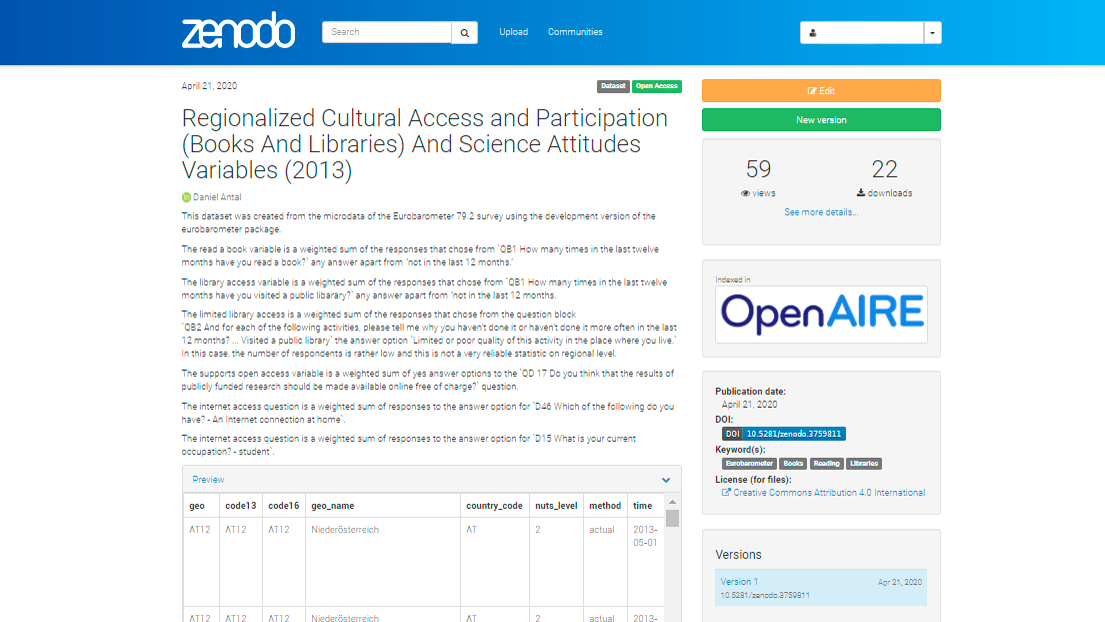
\includegraphics[width=15.35in]{plots/screenshots/zenodo_deposition_example} 

}

\caption{Zenodo Deposition Example}\label{fig:zenodo-example}
\end{figure}

You can see this dataset \href{https://zenodo.org/record/3759811\#.YJ6R3qgzbIU}{here}, which was used in \href{https://dataandlyrics.com/publication/scholarly_pirate_libraries_2020/}{this} high-profile scientific publication.

\hypertarget{deposit-indicator}{%
\section{Authentic Depositions of Indicators}\label{deposit-indicator}}

We designed a workflow that helps our curators to put their indicator tables to \href{https://zenodo.org/}{Zenodo}. In many cases, particularly if they do EU-funded research, this is also usually a grant requirement. At the same time, we place the indicator to our database, and make it available on our data observatory's API.

With low-frequency data, such as annual data tables, we place all copies to Zenodo first, and then to the data API. In these cases, each new version of the indicator values (containing a new year, a new estimation, or a new country, a new observation unit) will have a new DOI version.

With high-frequency data, such as data tables that are refreshing daily or several times a day, we do not think that authentic versioning is useful. In such cases, we create an authentic version at a pre-agreed time frequency, for example, monthly.

\hypertarget{how-to-add-your-existing-zenodo-depositions-to-our-observatory}{%
\subsection{How to Add your Existing Zenodo Depositions to Our Observatory}\label{how-to-add-your-existing-zenodo-depositions-to-our-observatory}}

If you have a relevant dataset on Zenodo that should be featured in one of our observatories, or you are just uploading a new dataset, you should send it to our observatory \texttt{communities}. Communities are just collections that make your data easier to find and cite.

On your new or existing deposition, go to Edit, and you will find \texttt{Communities} right after \texttt{Files} and above \texttt{Upload\ Type}.

\begin{figure}

{\centering 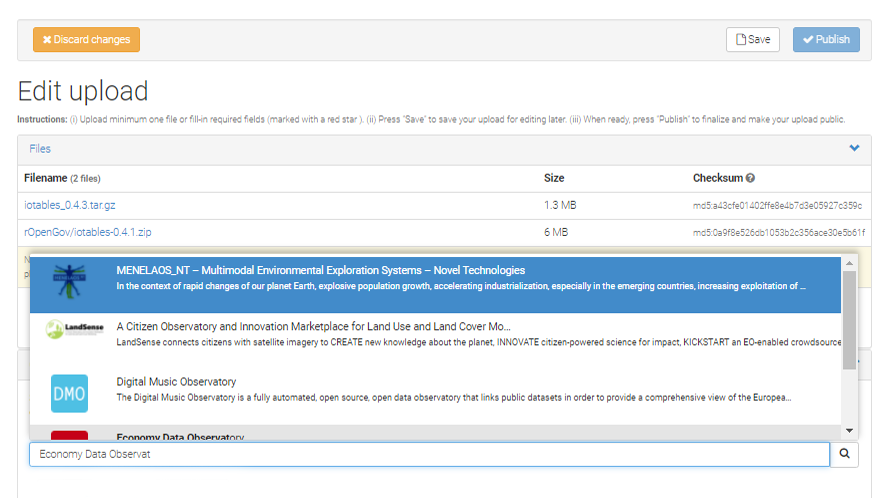
\includegraphics[width=0.85\linewidth]{plots/screenshots/zenodo_how_to_add} 

}

\caption{How to Add your Existing Zenodo Depositions to Our Observatory?}\label{fig:how-to-add-zenodo}
\end{figure}

If you want to be featured regularly in our observatories, your data should conform our database schema. In this case, we will help you maintaining the timeliness of your data -- basically we will together keep your dataset growing, expanding, and be available via our API, too. (See an example \href{http://34.226.91.55}{here}. We will add a tutorial on this shortly to our blog.)

\hypertarget{digital-music-observatory-1}{%
\subsubsection{Digital Music Observatory}\label{digital-music-observatory-1}}

You can deposit your data, or search for new, exciting data on Zenodo itself to our music observatory on \href{https://zenodo.org/communities/music_observatory?page=1\&size=20}{zenodo.org/communities/music\_observatory}.

\begin{figure}

{\centering 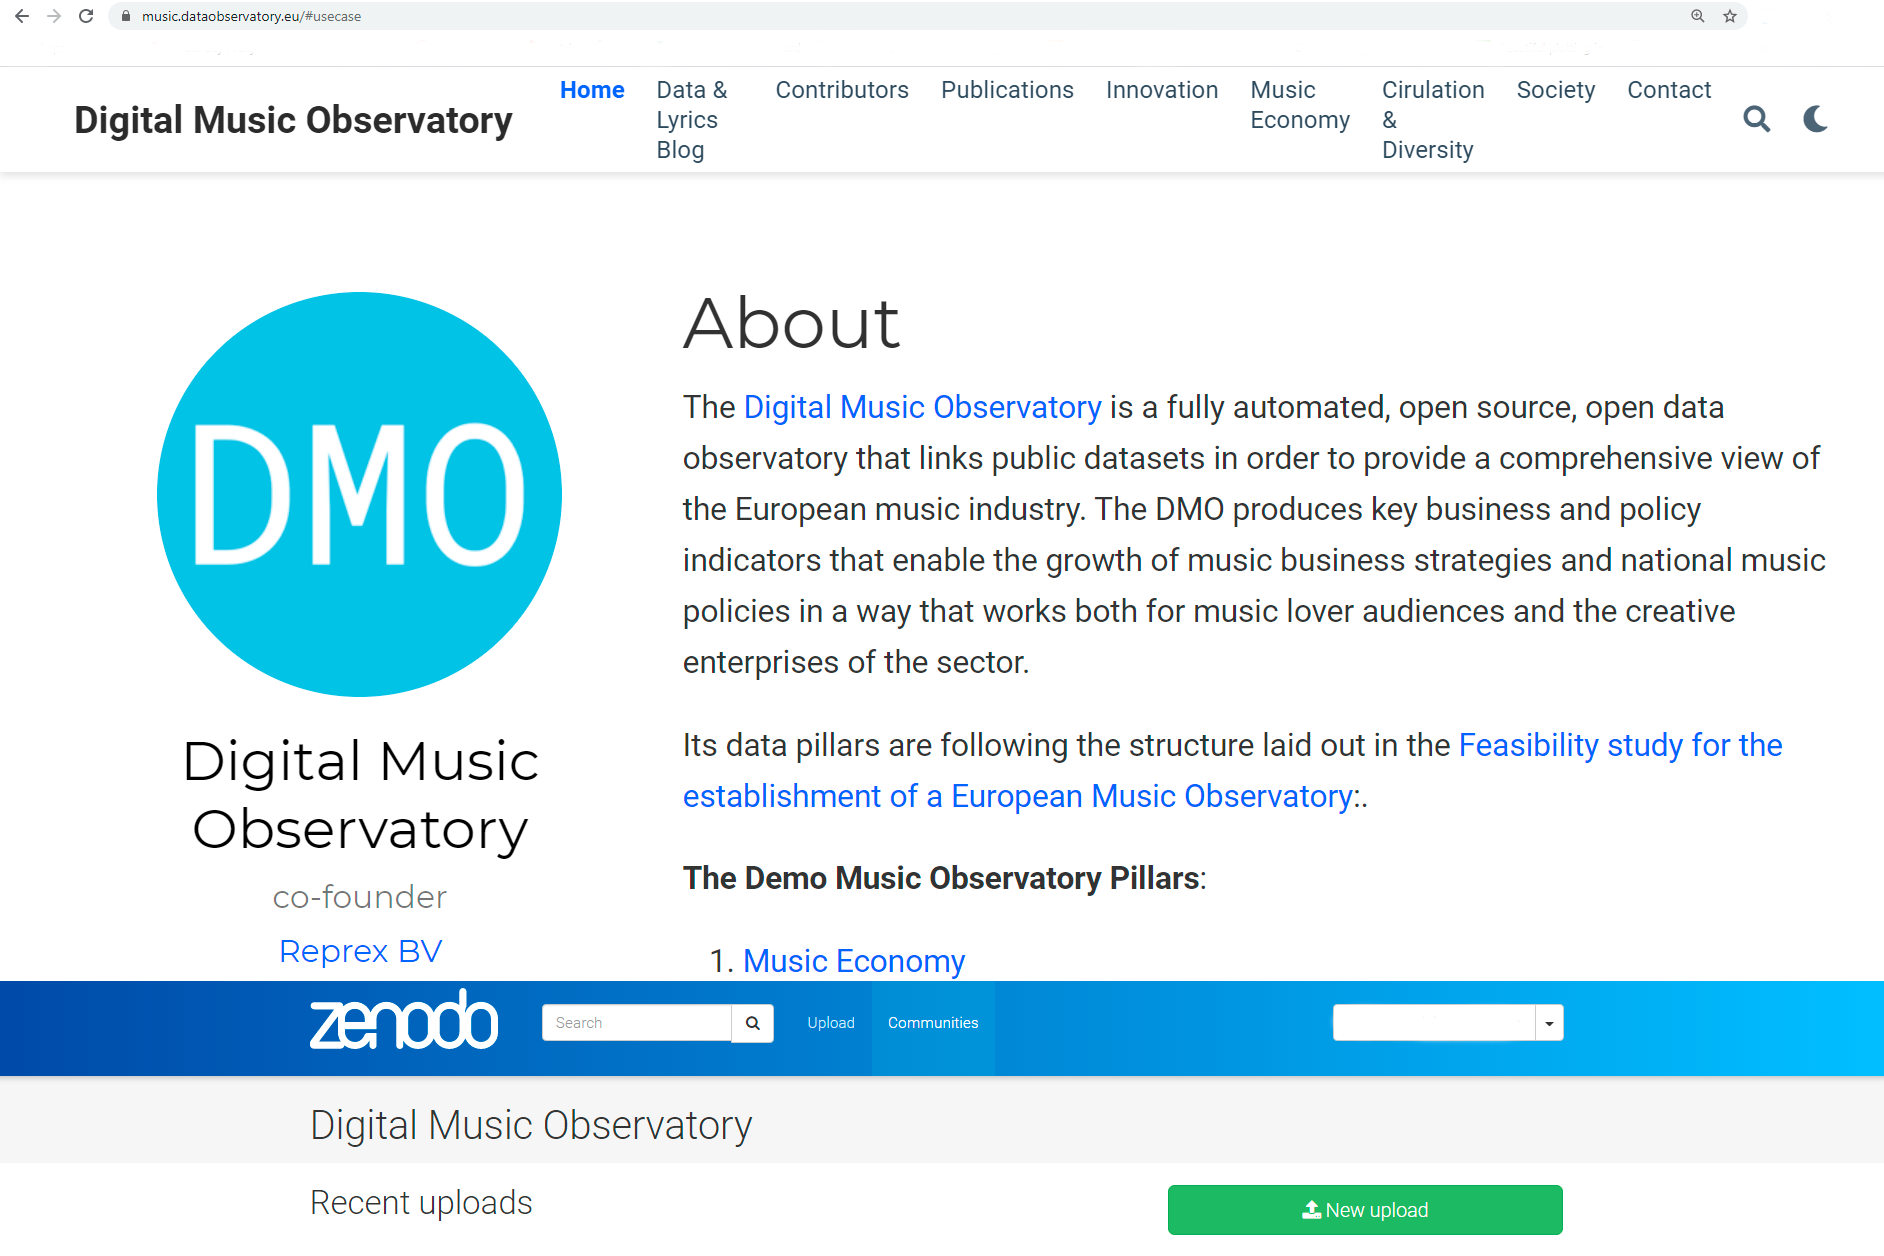
\includegraphics[width=0.85\linewidth]{plots/screenshots/dmo_and_zenodo} 

}

\caption{Deposit Data, Curate Data on Zenodo for the Digital Music Observatory}\label{fig:dmo-zenodo}
\end{figure}

\hypertarget{green-deal-data-observatory}{%
\subsection{Green Deal Data Observatory}\label{green-deal-data-observatory}}

You can deposit your data, or search for new, exciting data on Zenodo itself to our green deal data observatory on \href{https://zenodo.org/communities/greendeal_observatory?page=1\&size=20}{zenodo.org/communities/greendeal\_observatory}.

\begin{figure}

{\centering \includegraphics[width=0.85\linewidth]{plots/screenshots/greendeal_and_zenodo} 

}

\caption{Deposit Data, Curate Data on Zenodo for the Green Deal Data Observatory}\label{fig:greendeal-zenodo}
\end{figure}

\hypertarget{economy-data-observatory-1}{%
\subsubsection{Economy Data Observatory}\label{economy-data-observatory-1}}

You can deposit your data, or search for new, exciting data on Zenodo itself to our green deal data observatory on \href{https://zenodo.org/communities/economy_observatory?page=1\&size=20}{zenodo.org/communities/economy\_observatory/}.

\hypertarget{green-deal}{%
\chapter{Green Deal Indicators}\label{green-deal}}

Climate change and environmental degradation are an existential threat to Europe and the world. To overcome these challenges, the European Union created the European Green Deal strategic plan. It aims to make the EU's economy sustainable by turning climate and environmental challenges into opportunities, and making the transition just and inclusive for all.

Our data observatory is competing in the EU Datathon 2021. We believe that introducing Open Policy Analysis standards with open data, open-source software and research automation can help the Green Deal policymaking process. Our collaboration is open for individuals, citizens scientists, research institutes, NGOS, companies.

\begin{center}\includegraphics[width=26.32in]{plots/screenshots/greendeal_and_zenodo} \end{center}

Please, follow us on social media, it really helps us finding new users and showing that we are able to grow our ecosystem: the \href{https://www.linkedin.com/company/78556699}{Green Deal Data Observatory on Linkedin} and the \href{https://twitter.com/GreenDealObs}{Green Deal Data Observatory on Twitter}.

\hypertarget{curators}{%
\section{Curators}\label{curators}}

\begin{itemize}
\tightlist
\item
  \href{https://greendeal.dataobservatory.eu/post/2021-06-08-data-curator-karel-volckaert/}{Karel Volckaert: Credibility is Enhanced Through Cross Links Between Different Data from Different Domains}
\item
  \href{https://greendeal.dataobservatory.eu/post/2021-06-07-introducing-suzan-sidal/}{Suzan Sidal: We Need More Reliable Datasets on the Urban Heat Resilience and Disaster Risk Reduction}
\end{itemize}

See our \href{\%7B\#get-inspired\%7D}{inspirational examples} and \protect\hyperlink{first-contribution}{Your First Data Contribution} in the \ref{curators} chapter.

\hypertarget{aggregating-count-data}{%
\section{Aggregating Count Data}\label{aggregating-count-data}}

\texttt{We\ need\ to\ improve\ conservation\ by\ improving\ wildlife\ monitoring.\ Counting\ plants\ and\ animals\ is\ really\ tricky\ business.}

\begin{quote}
The marbled murrelet is an enigma. It wasn't until the 1970s that biologists discovered where the chunky brown-and-white bird made its home, and even then it was by accident: A tree-climber found a murrelet chick at the top of a redwood. Most other bird habitats had been mapped for centuries. But who would have thought to look for a sea bird's nest miles away in the middle of an old-growth forest?
And it's elusive. California birders can go a lifetime without seeing one. Every day at the break of dawn, the murrelet zips down from the redwood forest hills, where it lives, to the ocean, where it feeds. It then returns under the cover of darkness.
Using remote acoustic sensors and machine learning to analyze the audio, biologists are now better able to track populations of species that were previously hard to monitor. With a \href{https://www.fws.gov/arcata/es/birds/MM/m_murrelet.html}{threatened species} like the marbled murrelet, that can make a huge difference. The better the data on its population and nesting patterns, the better our understanding of how its habitat is threatened, and the more effective conservation efforts can be.
\end{quote}

\begin{figure}

{\centering 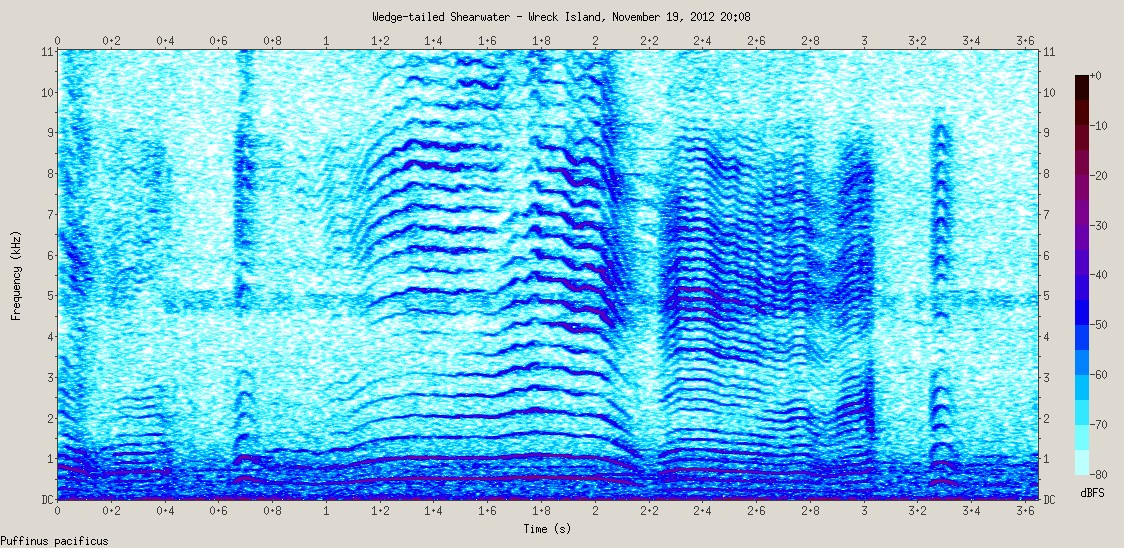
\includegraphics[width=0.8\linewidth]{plots/greendeal/wedgetailedshearwater} 

}

\caption{Soundscape of the Wedge-Tailed Shearwater from the Acoustic Metrics database}\label{fig:wedgetailedshearwater}
\end{figure}

\href{https://fivethirtyeight.com/features/big-data-is-saving-this-little-bird/}{Big Data Is Saving This Little Bird} -listen to the interview \href{https://podcasts.apple.com/us/podcast/17-little-bird-big-data/id1011406983?i=1000391467965}{here}. \emph{The illustration is taken from Jody Avirgan's blogpost.}

To analyze governmental, social data with ecological data, we need to place them on the same map. Biostatisticians, ecologists often work with count data -- counting trees, birds, various species. We need to aggregate count data over the same maps that statisticians use to count people, measure the GDP or make environmental and urban planning.

This knowledge is also very important for small area statistics that we apply in \protect\hyperlink{social-attitude-climate-change}{Social Attituted to Climate Change}

\hypertarget{social-attitude-climate-change}{%
\section{Social Attituted to Climate Change}\label{social-attitude-climate-change}}

what do people think about climate change in Europe and other parts of the world? Do they believe that the climate is changing? How? What they think about the causes? Do they report that they change their behavior? Teach their children to do so?

Please take a look at our blogpost \href{http://greendeal.dataobservatory.eu/post/2021-04-23-belgium-flood-insurance/}{Is Drought Risk Uninsurable?} as an example.

As a data curator:

\begin{itemize}
\tightlist
\item
  You identify openly accessible surveys that are harmonized (use standardized questions.) In our tutorial we projected the public opinion data from Eurobarometer 90.2 (fieldwork: October-November 2018.) on the municipal map of Belgium
\item
  Tell us which question items would be good candidates to report. We used the answers to the multiple choice question \texttt{QB1\ Do\ you\ think\ that\ the\ following\ extreme\ weather\ events\ are\ due\ to\ climate\ change?} We highlighted areas where people find it more likely to be exposed to \texttt{Droughts\ and\ wildfires}
\item
  How we should calculate the indicator? Take a certain answer and average it over a region? Weight the answers? How?
\item
  You write at least 1-2 unit tests: what must we check when the calculation is over. No negative numbers? Number of regions must up to 265?
\end{itemize}

If you write R code, you can get involved in our suvey harmonization and regional coding efforts.

See our tutorial:

\href{http://greendeal.dataobservatory.eu/post/2021-03-06-regions-climate/}{Regional Geocoding Harmonization Case Study - Regional Climate Change Awareness Datasets}

\begin{figure}

{\centering 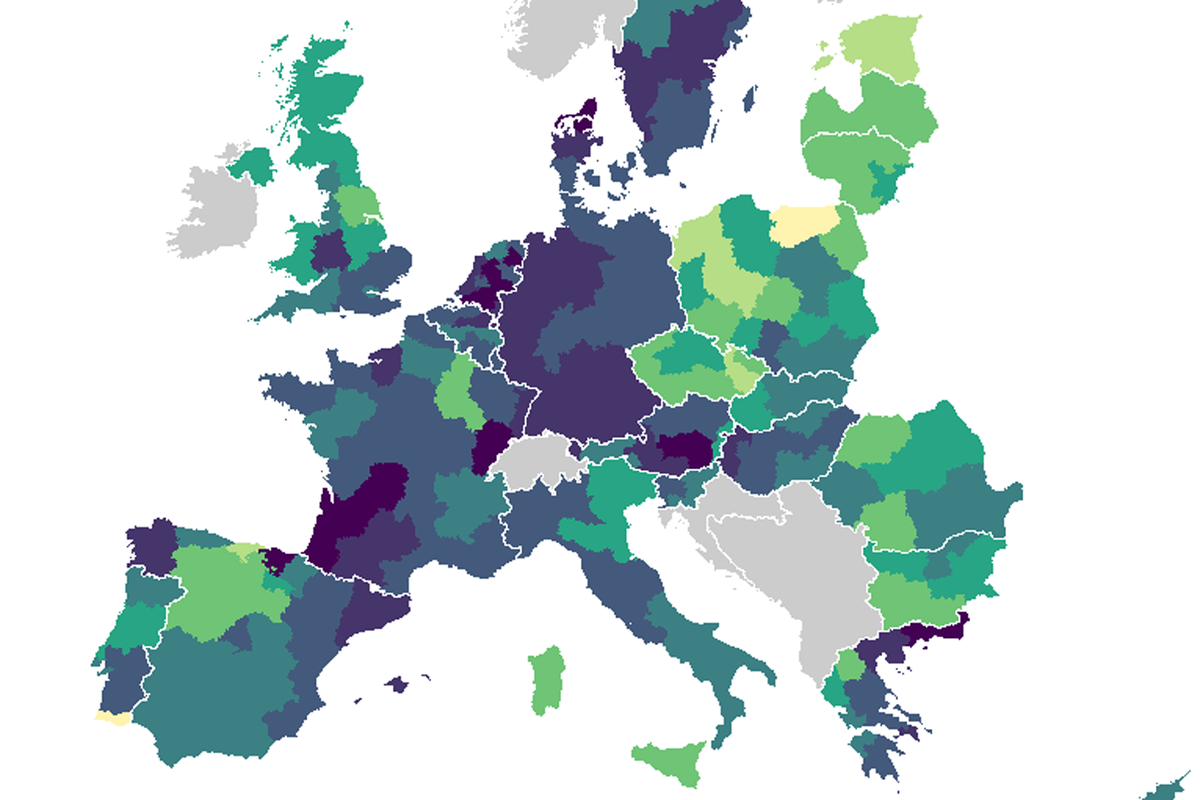
\includegraphics[width=0.67\linewidth]{plots/eurobarometer_climate_attitude_tutorial} 

}

\caption{Regional attituteds to climate change, from our survey regionalization tutorial}\label{fig:regional-climate-attitutes-tutorial}
\end{figure}

\hypertarget{environmental-impact-indicator-for-economic-activities}{%
\section{Environmental Impact Indicator for Economic Activities}\label{environmental-impact-indicator-for-economic-activities}}

Our \href{https://iotables.dataobservatory.eu/}{iotables} package practically implements The \href{https://ec.europa.eu/eurostat/en/web/products-manuals-and-guidelines/-/KS-RA-07-013}{Eurostat Manual of Supply, Use and Input-Output Tables} with real life data and in R, and it is checked against the published results from \href{http://ec.europa.eu/eurostat/documents/3859598/5902113/KS-RA-07-013-EN.PDF/b0b3d71e-3930-4442-94be-70b36cea9b39?version=1.0}{Jörg Beutel} (the author of this excellent manual), the Spicosa Project Report, and official UK statistical tables.

We used it to calculate the effects of cultural activities on various economies, but this methodology is particularly well-suited to measure the effects, or predict the effects of policy changes on greenhouse gas or pollutant emissions.

As a data curator:

\begin{itemize}
\tightlist
\item
  You identify openly accessible surveys data that can contains environmental effects for industries (Eurostat publishes them for many pollutants and greenhouse gases from the European Environmental Data.)
\item
  Tell us which particular data table would be good candidate to report. Give us ideas how to bridge various problems. (The SIOT matrix must be 60x60 or 64x64), sometimes industries must be added together.
\item
  If you write R code, we help you make the calculation yourself, if not, we'll take over.\\
\item
  Please assess the results with us, and let's publish them regularly. (Some EU member states update their SIOTs every year, others every 5 years, but pollutant data may be available annually.)
\end{itemize}

\hypertarget{sensory-data-measuring-climate-change-physical-affects}{%
\section{Sensory Data Measuring Climate Change Physical Affects}\label{sensory-data-measuring-climate-change-physical-affects}}

\hypertarget{music}{%
\chapter{Digital Music Observatory}\label{music}}

The \href{https://music.dataobservatory.eu/}{Digital Music Observatory} is a fully automated, open source, open data observatory that creates public datasets to provide a comprehensive view of the European music industry. It provides high-quality and timely indicators in all four pillars of the planned official European Music Observatory as a modern, open source and largely open data-based, automated, API-supported alternative solution for this planned observatory. The insight and methodologies we are refining in the DMO are applicable and transferable to about 60 other data observatories funded by the EU which do not currently employ governmental or scientific open data.

\begin{center}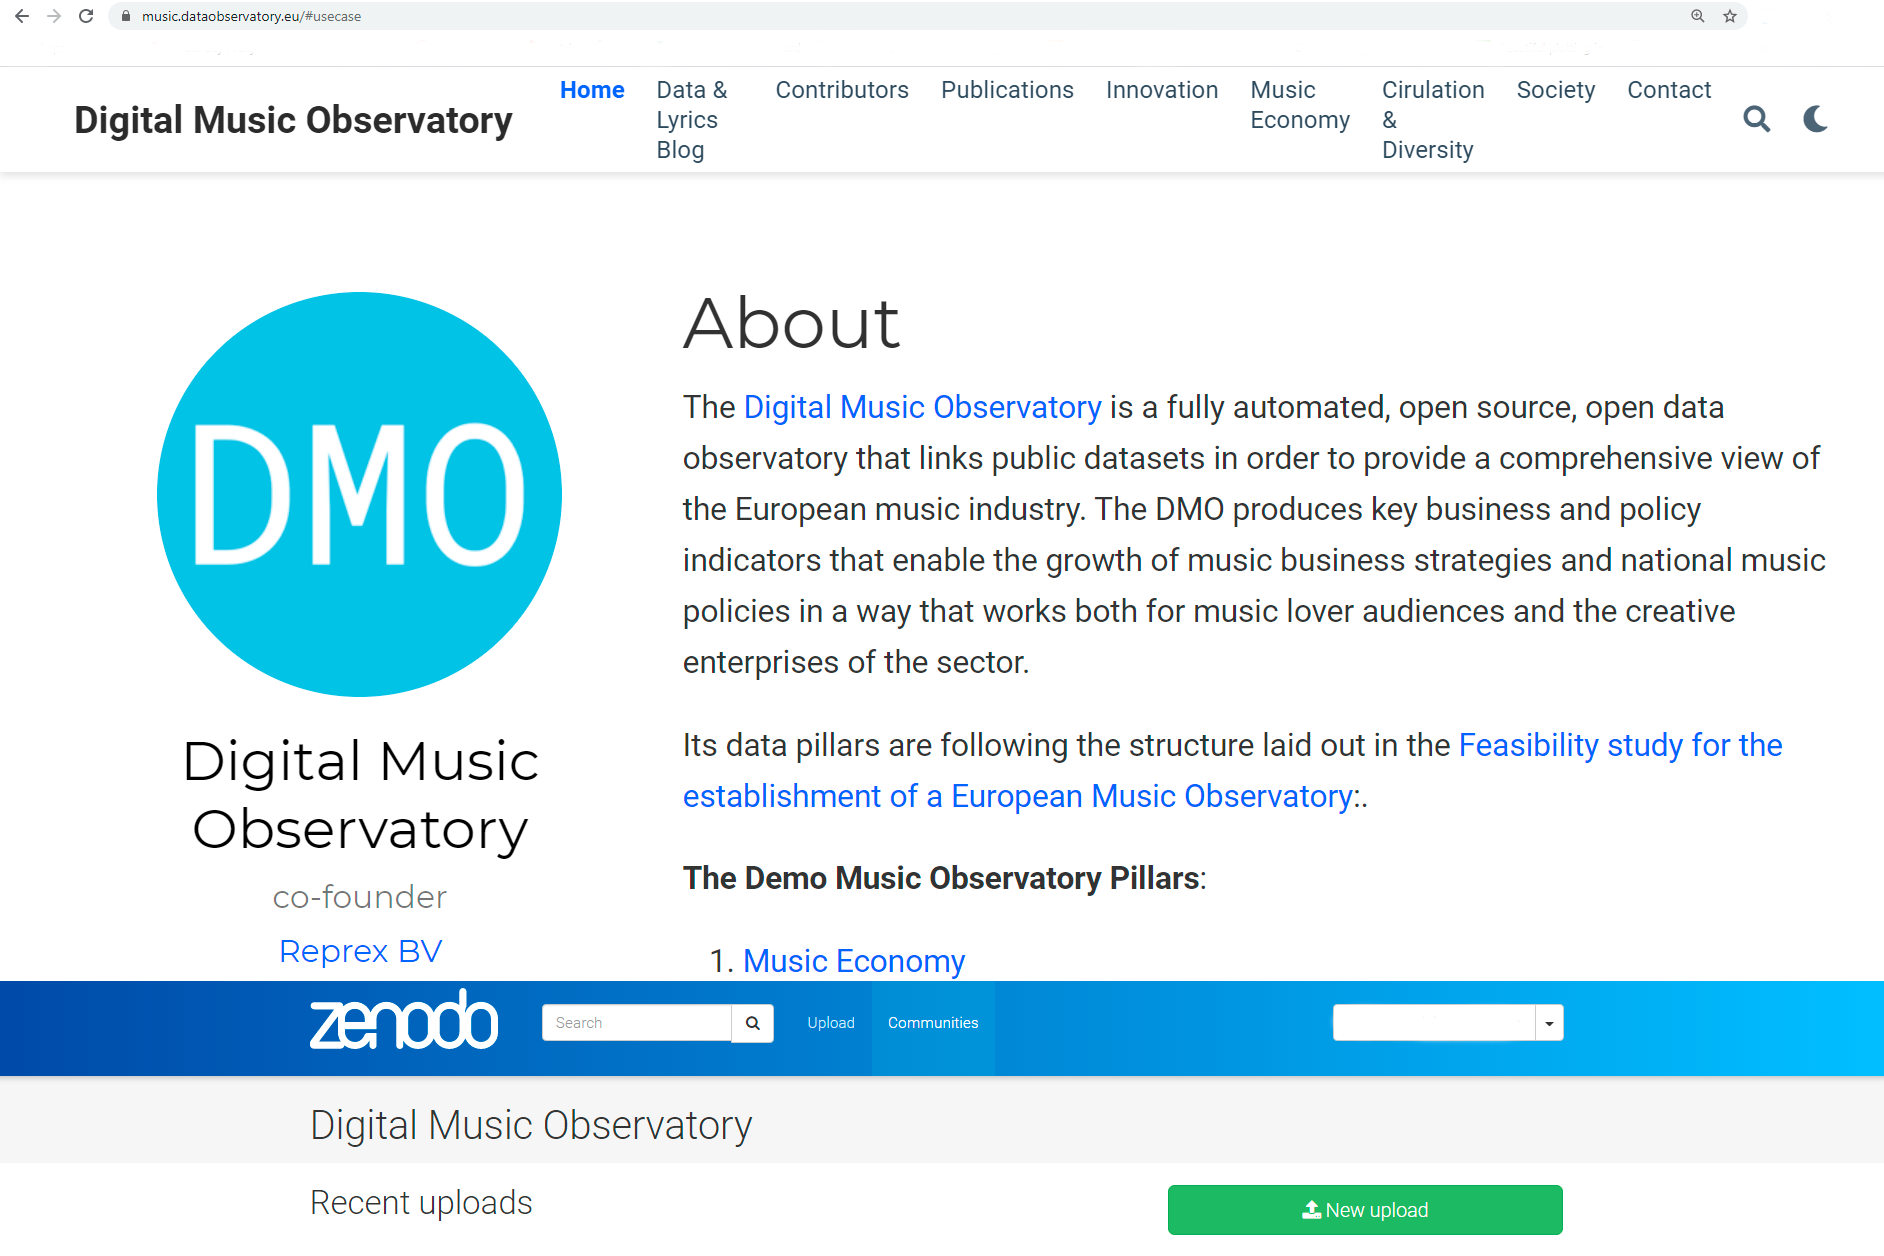
\includegraphics[width=26.17in]{plots/screenshots/dmo_and_zenodo} \end{center}

Music is one of the most data-driven service industries where the majority of sales are already made by AI-driven autonomous systems. We provide a template that enables making these AI-driven systems accountable and trustworthy, with the goal of re-balancing the legitimate interests of creators and consumers. Music, like all creative industries, can create high-value, human jobs in the future that utilize digital skills and human creativity. Within Europe, this new balance will be an important use case of the European Data Strategy and the Digital Services Act.

The DMO places the values of the European Data Strategy at its center: our observatory model allows the seamless flow of data within the EU and across sectors; it abides by European rules concerning privacy, access, and use; it pools data from a wide range of industries and sectors and makes it available for further research. The music industry is a global industry, and the best known European music scene in the world is the British. Our observatory aims to support a new relationship between the European and the UK music industries while offering international open data products from global sources.

The DMO is a fully-functional service that can function as a testing ground of the European Data Strategy, showcasing the ways in which the music industry is affected by the problems that the Digital Services Act and European Trustworthy AI initiatives attempt to regulate. Our observatory's policy insights also shed new light on important aspects of the Digital Skills and Connectivity agenda of the European Union. As a user-friendly one-stop shop for all things concerning data and the music industry, our DMO provides the foundations for a healthier and accountable European music ecosystem.

Please, follow us on social media, it really helps us finding new users and showing that we are able to grow our ecosystem: the \href{https://www.linkedin.com/company/reprexbv/}{Digital Music Data Observatory on Linkedin} and the \href{https://twitter.com/dataandlyrics}{Digital Music Data Observatory on Twitter}.

\hypertarget{music-curators}{%
\section{Curators}\label{music-curators}}

\begin{itemize}
\item
  \href{https://music.dataobservatory.eu/post/2021-06-02-data-curator-eszter-kabai/}{Eszter Kabai: New Indicators for Royalty Pricing and Music Antitrust}
\item
  \href{https://music.dataobservatory.eu/author/dominika-semanakova/}{Dominika Semaňáková: We Want Machine Learning Algorithms to Learn More About Slovak Music}
\end{itemize}

See our \href{\%7B\#get-inspired\%7D}{inspirational examples} and \protect\hyperlink{first-contribution}{Your First Data Contribution} in the \ref{curators} chapter.

\hypertarget{music-economy}{%
\section{Music Economy}\label{music-economy}}

\hypertarget{demand-drivers}{%
\subsection{Demand Drivers}\label{demand-drivers}}

Our music economy \href{https://data.music.dataobservatory.eu/music-economy.html}{demand drivers} are data that are known to be leading indicators to an increase in mechanical copies, streaming subscriptions, public performance use, private copying or illegal use of music.

\hypertarget{supply-indicators}{%
\subsection{Supply Indicators}\label{supply-indicators}}

Our Music Economy / \href{https://data.music.dataobservatory.eu/music-economy.html\#supply}{Supply} indicators are related to the supply of new music.

\hypertarget{price-indicators}{%
\subsection{Price Indicators}\label{price-indicators}}

\hypertarget{music-diversity}{%
\section{Music Diversity}\label{music-diversity}}

\hypertarget{gender-language-ethnic-and-other-inclusion-attributes}{%
\subsection{Gender, Language, Ethnic and Other Inclusion Attributes}\label{gender-language-ethnic-and-other-inclusion-attributes}}

\hypertarget{music-circulation}{%
\section{Music Circulation}\label{music-circulation}}

\hypertarget{market-shares}{%
\subsection{Market shares}\label{market-shares}}

We are developing \href{https://data.music.dataobservatory.eu/music-diversity.html\#cross-border-circulation-of-works}{market share} indicators for streaming and broadcast music.

For national, gender or other market share, we need to label both music works and recorded fixations. We use various open source databases, and machine learning algorithms to do prepare the data, but eventually our data goes through human musicology or music journalist curators.

For example, in our case study we were interested in the various definitions of \texttt{Slovak\ market\ share}, and representation of \texttt{female\ artists.} Both problems require rather challenging labeling.

\begin{enumerate}
\def\labelenumi{\alph{enumi})}
\tightlist
\item
  we tried to find a location to the artist / band {[} you can describe why this is not always straightforward, for example, in the case of dead artists, etc.{]}
\item
  our algorithm tried to guess the language of the 10 most popular song titles
\item
  we checked if the person is on the Wikipedia list of ``Slovak male singers'', ``Slovak female singers'', ``Slovak bands'', or their Czechoslovak versions {[} who did you decide when somebody was Czechoslovak if they were Slovak{]}
\item
  check if there was a Slovak placename mentioned on their bandcamp site
\item
  check if they are associated with Slovakia on the Musicbrainz open source database
\item
  if any of the artists released recodings was released in Slovakia
\item
  if the majority of the artist's released recordings was released in Slovakia
\end{enumerate}

\ldots.

Until we got to the human curation.

and eventually we either \texttt{considered\_slovak} or not somebody in our \texttt{write-in\ database}. We are also developing an \texttt{opt-in\ database}, where artists can give us their own ethnic, local and gender identity, if they wish to, and of course, they can opt-out from our labeling.

We are using Monte Carlo simulation and non-parametric sampling of various broadcast and music streams to get a representation of the music listened to in various cities, regions, countries, and then we apply \texttt{national}, \texttt{language}, \texttt{gender}, \texttt{sex}, \texttt{locality} and \texttt{folksonomy} tags to measure female, Slovak, Estonian, Amsterdam or Welsh market share, recommendation probability, etc.

\hypertarget{music-society}{%
\section{Music \& Society}\label{music-society}}

\hypertarget{social-attitutes-to-music}{%
\subsection{Social Attitutes to Music}\label{social-attitutes-to-music}}

\hypertarget{participation-in-music}{%
\subsection{Participation in Music}\label{participation-in-music}}

\hypertarget{economy}{%
\chapter{Economy Data Observatory}\label{economy}}

Big data and automation create new inequalities and injustices and has a potential to create a jobless growth. Our Economy Observatory is a fully automated, open source, open data observatory that produces new indicators from open data sources and experimental big data sources, with authoritative copies and a modern API.

Our observatory is monitoring the European economy to protect the consumers and the small companies from unfair competition both from data and knowledge monopolization and robotization. We take a critical SME-, intellectual property policy and competition policy point of view automation, robotization, and the AI revolution on the service-oriented European social market economy.

We would like to create early-warning, risk, economic effect, and impact indicators that can be used in scientific, business and policy contexts for professionals who are working on re-setting the European economy after a devastating pandemic and in the age of AI. We are particularly interested in designing indicators that can be early warnings for killer acquisitions, algorithmic and offline discrimination against consumers based on nationality or place of residence, signs of undermining key economic and competition policy goals, and generally help small and medium-sized enterprises and start-ups to grow, and the financial sector to provide loanable and equity funds for their growth.

\begin{center}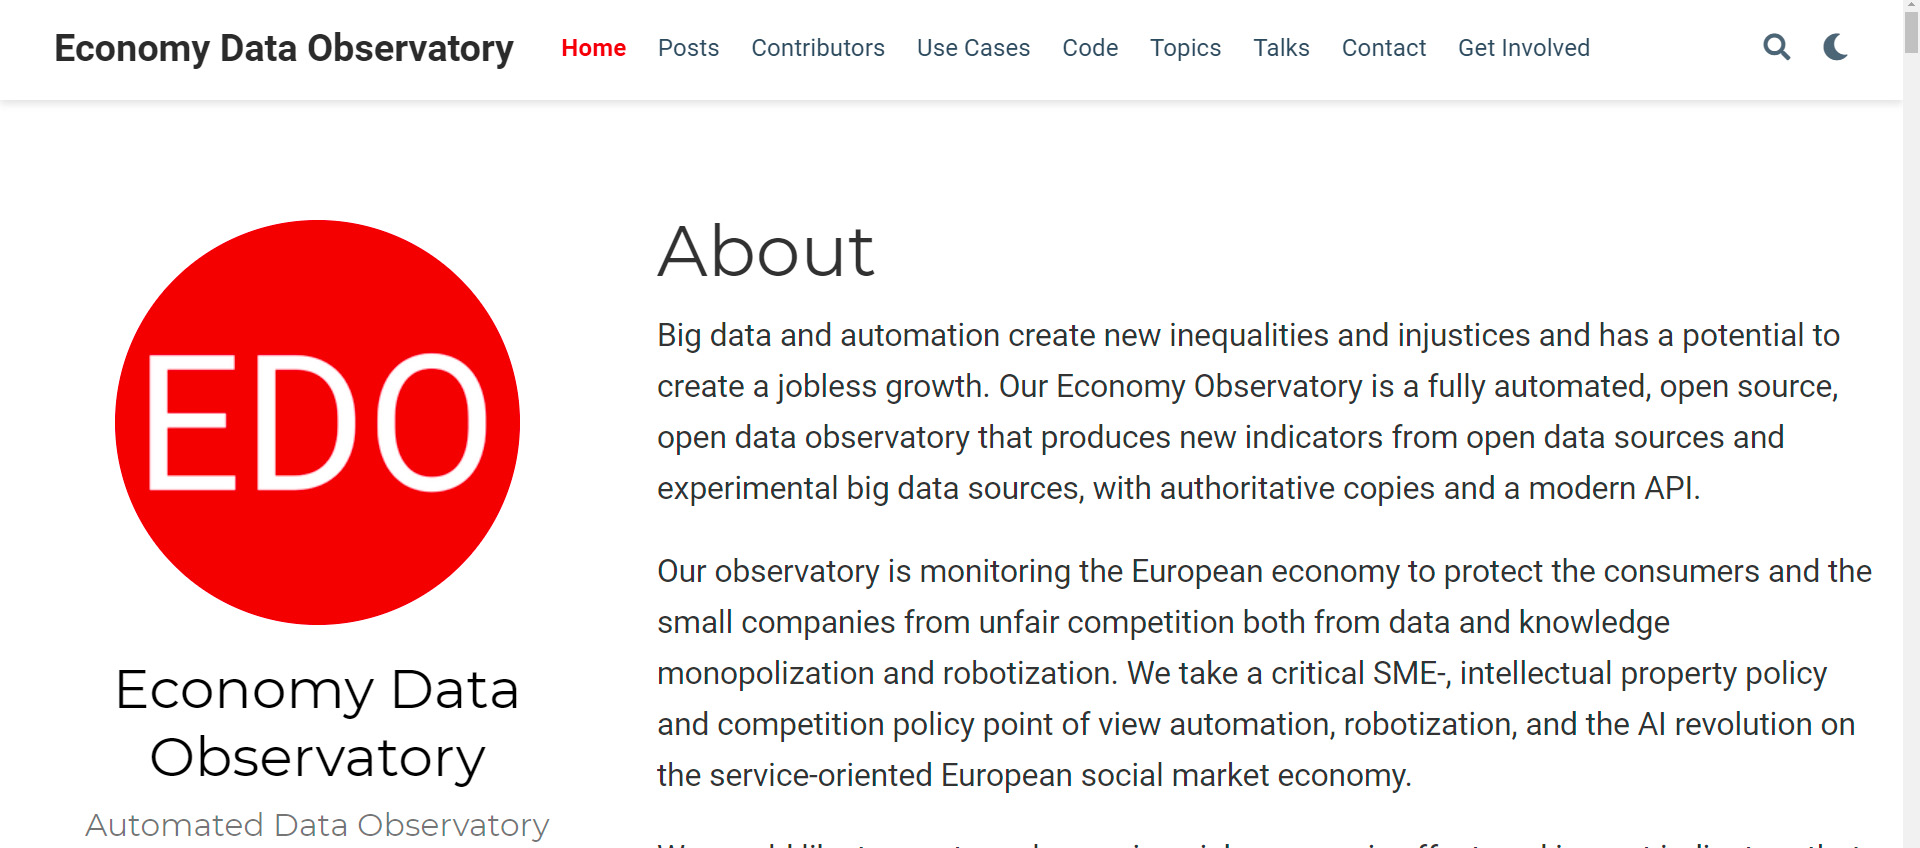
\includegraphics[width=26.67in]{plots/screenshots/edo_opening_page} \end{center}

\begin{quote}
An important aspect of the EU Datathon Challenges is ``.. to propose the development of an application that links and uses open datasets {[}\ldots{]} to find suitable new approaches and solutions to help Europe achieve important goals set by the European Commission through the use of open data.''
\end{quote}

In the \href{https://ec.europa.eu/info/strategy/priorities-2019-2024/economy-works-people_en\#:~:text=Individuals\%20and\%20businesses\%20in\%20the,needs\%20of\%20the\%20EU's\%20citizens.}{An economy that works for people} challenge we are focusing on the \href{https://ec.europa.eu/info/strategy/priorities-2019-2024/economy-works-people/internal-market_en}{Single market strategy}, and particular attention to the strategy's goals of 1. Modernising our standards system, 2. Consolidating Europe's intellectual property framework, and 3. Enabling the balanced development of the collaborative economy strategic goals.

\begin{center}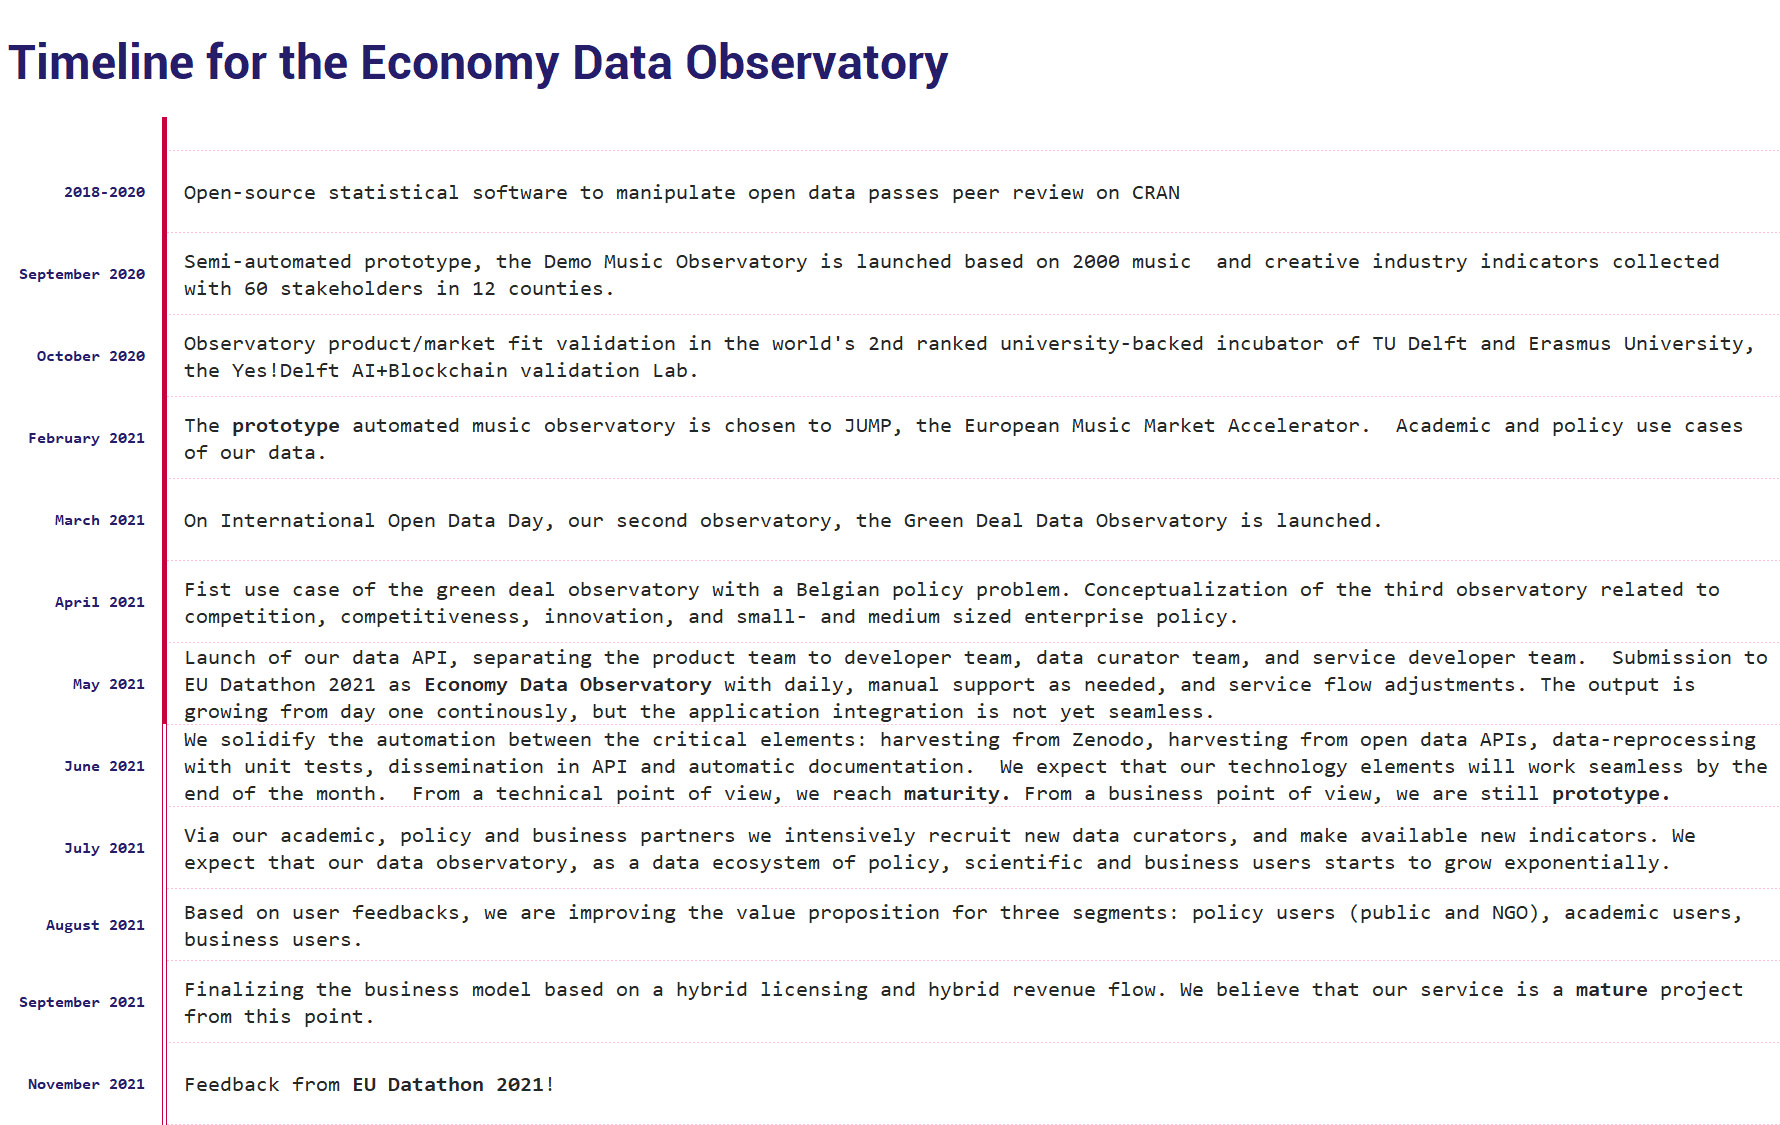
\includegraphics[width=24.72in]{plots/screenshots/Economy_Data_Observatory_timeline} \end{center}

\hypertarget{curators-1}{%
\section{Curators}\label{curators-1}}

\href{https://economy.dataobservatory.eu/post/2021-06-02-data-curator-peter-ormosi/}{Peter Ormosi: New Indicators for Computational Antitrust}

See our \href{\%7B\#get-inspired\%7D}{inspirational examples} and \protect\hyperlink{first-contribution}{Your First Data Contribution} in the \ref{curators} chapter.

\hypertarget{social-attitutes-to-economic-change}{%
\section{Social Attitutes to Economic Change}\label{social-attitutes-to-economic-change}}

what do people think about climate change in Europe and other parts of the world? Do they believe that the climate is changing? How? What they think about the causes? Do they report that they change their behavior? Teach their children to do so?

Please take a look at our blogpost \href{http://greendeal.dataobservatory.eu/post/2021-04-23-belgium-flood-insurance/}{Is Drought Risk Uninsurable?} as an example.

As a data curator:

\begin{itemize}
\tightlist
\item
  You identify openly accessible surveys that are harmonized (use standardized questions.) In our tutorial we projected the public opinion data from Eurobarometer 90.2 (fieldwork: October-November 2018.) on the municipal map of Belgium
\item
  Tell us which question items would be good candidates to report. We used the answers to the multiple choice question \texttt{QB1\ Do\ you\ think\ that\ the\ following\ extreme\ weather\ events\ are\ due\ to\ climate\ change?} We highlighted areas where people find it more likely to be exposed to \texttt{Droughts\ and\ wildfires}
\item
  How we should calculate the indicator? Take a certain answer and average it over a region? Weight the answers? How?
\item
  You write at least 1-2 unit tests: what must we check when the calculation is over. No negative numbers? Number of regions must up to 265?
\end{itemize}

If you write R code, you can get involved in our suvey harmonization and regional coding efforts.

See our tutorial:

\href{http://greendeal.dataobservatory.eu/post/2021-03-06-regions-climate/}{Regional Geocoding Harmonization Case Study - Regional Climate Change Awareness Datasets}

\begin{figure}

{\centering 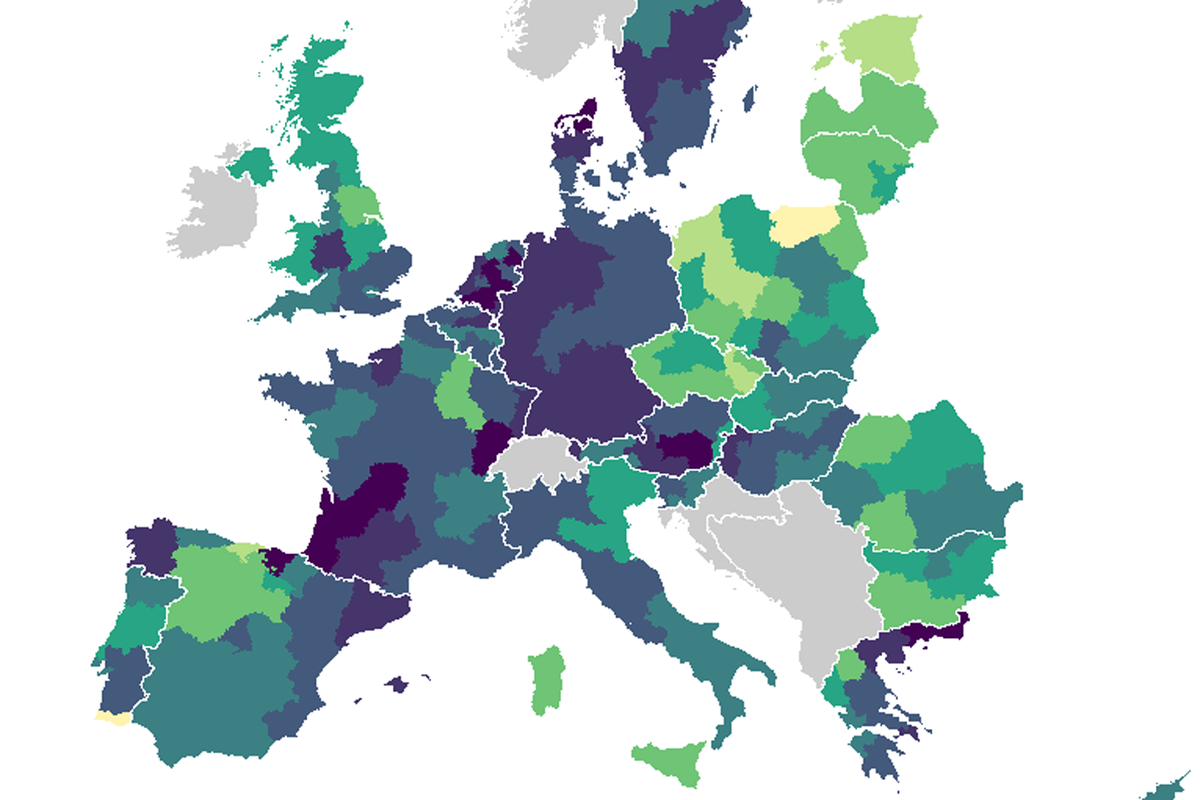
\includegraphics[width=0.67\linewidth]{plots/eurobarometer_climate_attitude_tutorial} 

}

\caption{Regional attituteds to climate change, from our survey regionalization tutorial}\label{fig:regional-climate-attitutes-tutorial-2}
\end{figure}

\hypertarget{sme-indicators}{%
\section{SME Activity Indicators}\label{sme-indicators}}

\hypertarget{economic-impact-indicators}{%
\section{Economic Impact Indicators}\label{economic-impact-indicators}}

Our \href{https://iotables.dataobservatory.eu/}{iotables} package practically implements The \href{https://ec.europa.eu/eurostat/en/web/products-manuals-and-guidelines/-/KS-RA-07-013}{Eurostat Manual of Supply, Use and Input-Output Tables} with real life data and in R, and it is checked against the published results from \href{http://ec.europa.eu/eurostat/documents/3859598/5902113/KS-RA-07-013-EN.PDF/b0b3d71e-3930-4442-94be-70b36cea9b39?version=1.0}{Jörg Beutel} (the author of this excellent manual), the Spicosa Project Report, and official UK statistical tables.

We used it to calculate the effects of cultural activities on various economies, but this methodology is particularly well-suited to measure the effects, or predict the effects of policy changes on greenhouse gas or pollutant emissions.

As a data curator:

\begin{itemize}
\tightlist
\item
  You identify openly accessible surveys data that can contains environmental effects for industries (Eurostat publishes them for many pollutants and greenhouse gases from the European Environmental Data.)
\item
  Tell us which particular data table would be good candidate to report. Give us ideas how to bridge various problems. (The SIOT matrix must be 60x60 or 64x64), sometimes industries must be added together.
\item
  If you write R code, we help you make the calculation yourself, if not, we'll take over.\\
\item
  Please assess the results with us, and let's publish them regularly. (Some EU member states update their SIOTs every year, others every 5 years, but pollutant data may be available annually.)
\end{itemize}

\hypertarget{sensory-data-measuring-changes-in-economic-activy}{%
\section{Sensory Data Measuring Changes in Economic Activy}\label{sensory-data-measuring-changes-in-economic-activy}}

\hypertarget{competition}{%
\chapter{Competition Data Observatory}\label{competition}}

Big data and automation create new inequalities and injustices and has a potential to create a jobless growth. Our Economy Observatory is a fully automated, open source, open data observatory that produces new indicators from open data sources and experimental big data sources, with authoritative copies and a modern API.

Our observatory is monitoring the European economy to protect the consumers and the small companies from unfair competition both from data and knowledge monopolization and robotization. We take a critical SME-, intellectual property policy and competition policy point of view automation, robotization, and the AI revolution on the service-oriented European social market economy.

We would like to create early-warning, risk, economic effect, and impact indicators that can be used in scientific, business and policy contexts for professionals who are working on re-setting the European economy after a devastating pandemic and in the age of AI. We are particularly interested in designing indicators that can be early warnings for killer acquisitions, algorithmic and offline discrimination against consumers based on nationality or place of residence, signs of undermining key economic and competition policy goals, and generally help small and medium-sized enterprises and start-ups to grow, and the financial sector to provide loanable and equity funds for their growth.

\begin{center}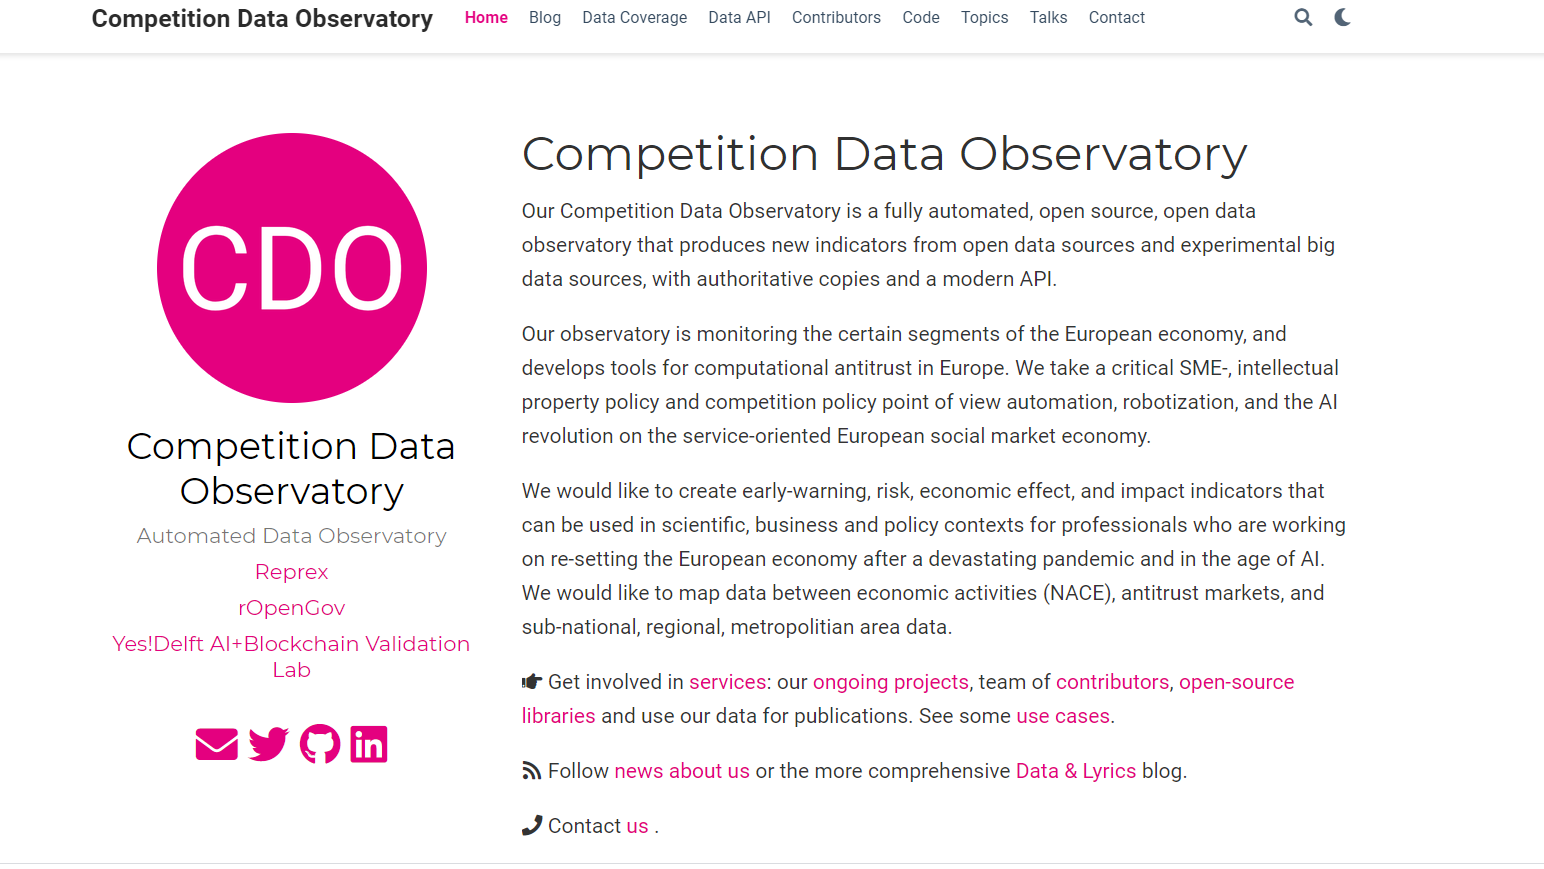
\includegraphics[width=21.44in]{C:/_bookdown/observatory_data_curators/plots/screenshots/cdo_opening_page} \end{center}

\hypertarget{competition-curators}{%
\section{Curators}\label{competition-curators}}

\href{https://economy.dataobservatory.eu/post/2021-06-02-data-curator-peter-ormosi/}{Peter Ormosi: New Indicators for Computational Antitrust}

See our \href{\%7B\#get-inspired\%7D}{inspirational examples} and \protect\hyperlink{first-contribution}{Your First Data Contribution} in the \ref{curators} chapter.

\hypertarget{compeition-indicators}{%
\section{Competition}\label{compeition-indicators}}

We are seeking API level access to the European Commissions Mergers database, and monitor approved and declined merger requests programatically. These mergers are important cases enough to have a potential impact on the structure of the European economy.

\begin{figure}

{\centering 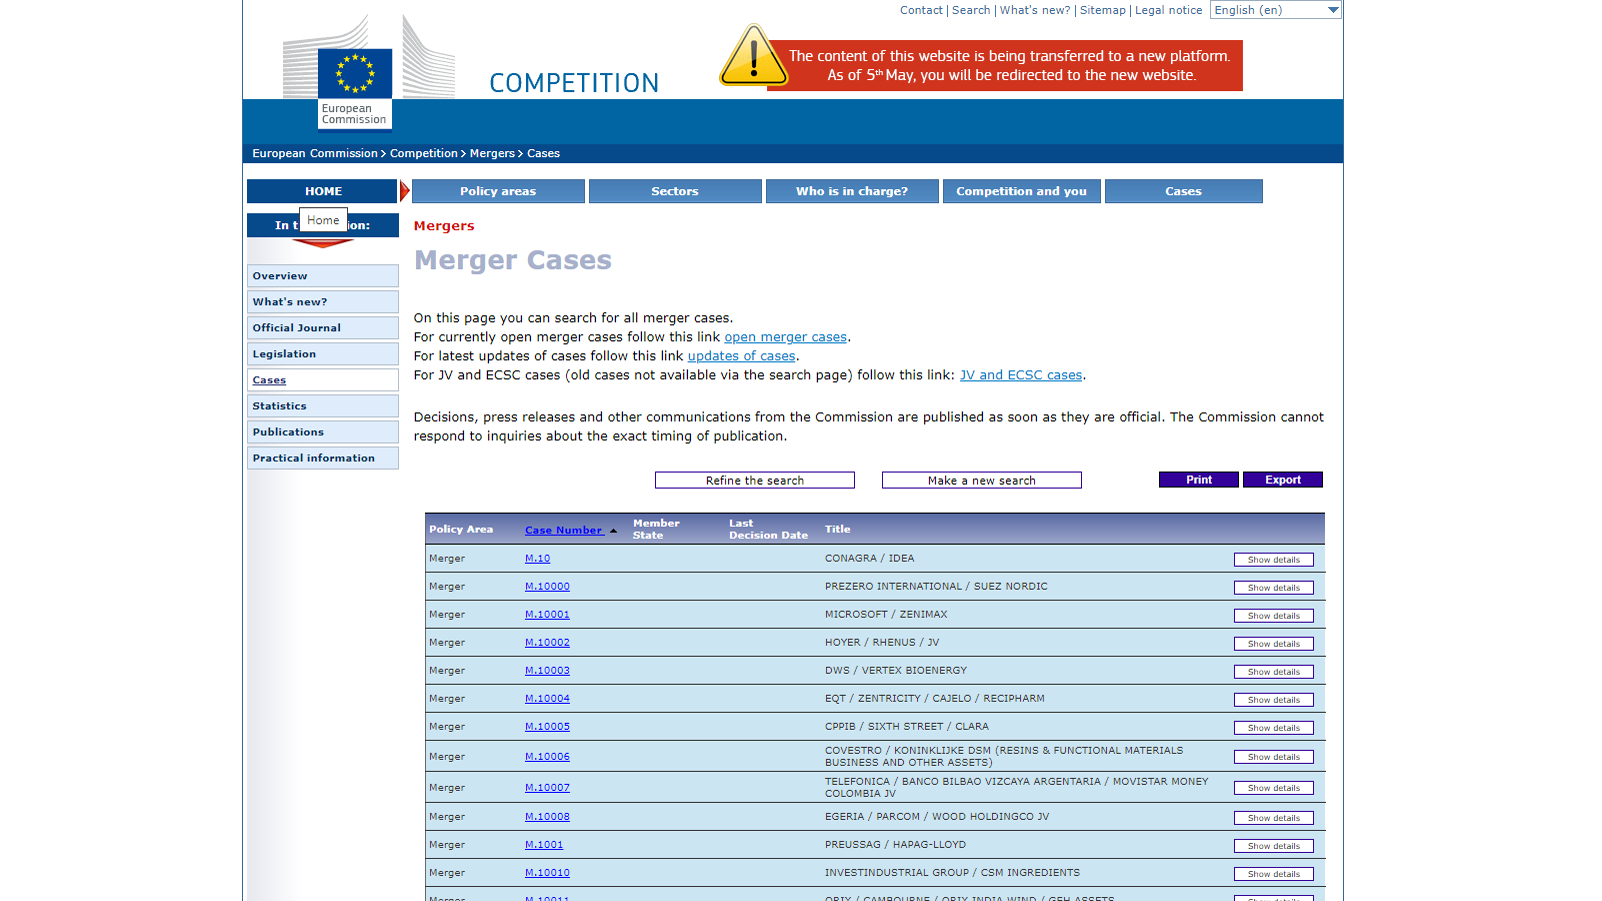
\includegraphics[width=0.8\linewidth]{plots/screenshots/ec_competition_merger_screenshot} 

}

\end{figure}

As a data curator, you help us designing datasets

\begin{itemize}
\tightlist
\item
  created from Commission and member state merger decision text databases (we will use NLP extraction from the text of the decisions)
\item
  top-down indicators that show the structural (concentration) changes in the European economy
\item
  connect them to patent databases
\end{itemize}

These indicators are particularly interestign, because we are trying to connect to databases that fall under the \href{https://eur-lex.europa.eu/legal-content/EN/TXT/?qid=1561563110433\&uri=CELEX:32019L1024}{Directive on open data and the re-use of public sector information - in short: Open Data Directive (EU) 2019 / 1024}, but programmatic access appears to be problematic. We need to secure reproducible, programmatic access to these important open data sources.

\hypertarget{knowledge-monopoly}{%
\subsection{Knowledge Monopolizations, Killer Acquisitions}\label{knowledge-monopoly}}

In killer acquisitions, a large company, for example, in pharmaceutical or technology fiedls, buys a small company, or even a start-up, to avoid disruptive innovation. We are building several types of indicators in this field.

\begin{itemize}
\tightlist
\item
  What type of patents companies hold in smaller entities of mergers and acquisitions? How can we characterize potentially disruptive technology?
\item
  Which economic activities (industries as describe by NACE) are more and less effected?
\item
  How is patent concentration changing?
\end{itemize}

\hypertarget{partnerships}{%
\chapter{Partnerships}\label{partnerships}}

We are looking for partners to develop our \protect\hyperlink{app}{technological solution} in \href{service}{financially sustainable way} with bringing more and more relevant, \protect\hyperlink{data-curators}{curated} open data \protect\hyperlink{open-data}{to light}.

\hypertarget{policy-partners}{%
\section{Policy Partners}\label{policy-partners}}

We are looking for policy partners who want to use open data from various governmental (including publicly funded surveys), scientific, and big data sources, processed and validated to meet scientific standards; or who want to build use cases for trustworthy AI and data governance policy papers. We provide peer-reviewed statistical software solutions, daily data harvesting, and re-processing to meet our partners' research agenda.

In return, we ask academic partners to:
1. Help us curate data -- tell us what sort of information is missing for their research agenda, and select what is valuable and what is not;
2. Use our validated, correctly documented, open datasets, identified with DOIs (possibly with an embargo period) in their peer-reviewed scientific output;
3. Support the growth of our data observatories by including them in their data acquisitions plans;
4. Publicly endorse with testimonials the observatory they use for the EU Datathon Prize.

\hypertarget{academic-partners}{%
\section{Academic Partners}\label{academic-partners}}

We are looking for academic partners who want to use open data from various governmental (including publicly funded surveys), scientific, and big data sources, processed and validated to meet scientific standards. We provide peer-reviewed statistical software solutions, daily data harvesting, and re-processing to meet our partners research agenda.

In return, we ask academic partners to

\begin{enumerate}
\def\labelenumi{\arabic{enumi}.}
\tightlist
\item
  Help us curate data -- tell us what sort of information is missing for their research agenda, and select what is valuable and what is not;
\item
  Use our validated, correctly documented, open datasets, identified with DOIs (possibly with an embargo period) in their peer-reviewed scientific output;
\item
  Support the growth of our data observatories by including them in their data acquisitions plans;
\item
  Publicly endorse with testimonials the observatory they use for the EU Datathlon Prize.
\end{enumerate}

\hypertarget{business-partners}{%
\section{Business Partners}\label{business-partners}}

"To take part, you should propose the development of an application that links and uses open datasets. Your application should showcase

We are looking for a consulting partner to form a joint project with our open collaboration team of data scientists and submit proposals to at least 2 of the 3 challenges of the EU Datathlon with the objective of winning the first prize. We are particularly looking for a first class consultancy to help build a ``showcase \ldots{} for concrete business models {[}\ldots{} and{]} find suitable new approaches and solutions to help Europe achieve important goals set by the European Commission through the use of {[}our observatories'{]} open data.''

Because of the way the challenge is formulated, winning the prize gives a natural advantage for our consulting partner to win future policy consulting work in the three strategic objective areas of the European Commission. Furthermore, we believe that our research automation technology and know-how can significantly reduce non-billable hours in research and validation, as well as in sales preparation and re-sale.

The partners of the Datathon Challenge are important EU and member state organizations, including the World Bank Group, FAO of the United Nations, the European Central Bank, the EU IP Office, and EFTA. We believe that winning this prize could give a competitive edge for our partners, given the high profile and rigor of the competition.

\hypertarget{tools}{%
\chapter{Tools}\label{tools}}

We do reproducible products. If it works once, it must work all the time, on Windows, Mac, Linux, in Word, PDF, html, using a laptop, a cloud server, a smartphone or a table.

\begin{itemize}
\item
  We use \protect\hyperlink{keybase}{Keybase} for internal communication
\item
  We are slowly bringing everybody on board with \protect\hyperlink{github}{Git} for online collaboration and file syncing. For a short time, we'll still use Google Docs.
\end{itemize}

If you work with us, you must adhere to the \href{https://www.contributor-covenant.org/version/2/0/code_of_conduct/}{Contributor Covenant}

The pledge starts with these paragraphs:

\emph{We as members, contributors, and leaders pledge to make participation in our community a harassment-free experience for everyone, regardless of age, body size, visible or invisible disability, ethnicity, sex characteristics, gender identity and expression, level of experience, education, socio-economic status, nationality, personal appearance, race, religion, or sexual identity and orientation.}

\emph{We pledge to act and interact in ways that contribute to an open, welcoming, diverse, inclusive, and healthy community.} Please, take the time to read once the entire \href{https://www.contributor-covenant.org/version/2/0/code_of_conduct/}{pledge}.

\hypertarget{internal-communication-collaboration}{%
\section{Internal communication \& collaboration}\label{internal-communication-collaboration}}

\hypertarget{keybase}{%
\subsection{Keybase}\label{keybase}}

No more long emails. Nobody's left out. No more misunderstandings. No more waiting for feedback.

\textbf{What do we need?}

\begin{itemize}
\item
  A simple-to-use communication tool where you can opt-in to be informed on a real time basis, or completely ignore us for days -- similar to Whatsapp Group, Microsoft Teams, Google Hangout, Slack;
\item
  A single, secure storage for shared documents -- similar to Google Drive, Microsoft One Drive, Dropbox;
\item
  An integration with Github -- a critical feature to at least the part of our team that is working on software code or long-form technical documentations;
\item
  Ability to oversee communications with more than 50 people with an option to streamline per topic, group, etc.;
\item
  To avoid using emails boxes, Whatsapp, Viber, etc. -- part-timers are not flooded with messages at all times, while full-timers can reach out to each other at any time;
\item
  A space where we can communicate all the time without interrupting calls and meetings with clients on other platforms;
  An integration to a project management tool that we will use for larger projects;
\item
  A tool as simple as possible, light touch;
\item
  Since we work in the open source, open data, open collaboration community, we would like to use something that is open source -- but we are willing to pay for solutions.
\end{itemize}

And the winner is\ldots.KEYBASE.IO

Keybase is a very neat, simple, lightweight team management / chat / social networking application that is extremely focused on privacy, security and encryption.

\textbf{Keybase Key features}

\begin{itemize}
\item
  Secure instant messaging, even with a timed self-destruction feature (e.g.~for sharing passwords);
  Starts a Google Meet or Zoom video call natively with a single command;
\item
  Brings your Whatsapp chat to the more private and secure keybase chat on the fly;
\item
  Team chat rooms in real time. You can filter where you want to be involved, and you can always opt-out;
\end{itemize}

-K-Drive (similar to OneDrive, Google Drive, Dropbox) -- only for our team, and fully encrypted;
Works with Github, and it even offers a more private version of Private Github Repos, encrypted gits;
An integration with other platforms;
It is neat, open source, simple, clean, and usually appreciated more in the open source community than Slack, its big corporation rival.

Practical steps you need to follow to use Keybase

\begin{enumerate}
\def\labelenumi{\arabic{enumi}.}
\tightlist
\item
  Download \& install Keybase from \url{https://keybase.io/} on your computer.
\end{enumerate}

An easy procedure. Create yourself a professional login name -- similarly to a professional github account, a professional email, etc. (you cannot change the name afterwards)

\begin{enumerate}
\def\labelenumi{\arabic{enumi}.}
\setcounter{enumi}{1}
\item
  Once you log in to the computer, go to \emph{Devices}, and \emph{Create a paper key}. Write this on paper, or print it, and store it somewhere very safe (not near your computer). This to recover the access in case you lose access to all your devices.
\item
  You can use Keybase simultaneously on multiple devices -- Install Keybase on your smartphone, tablet or any other device. You will be guided through installation \& paired with your computer.
\item
  Shall you need them, you have \emph{two recovery options}: the paper key and your smartphone.
\item
  If your smartphone breaks down and needs a replacement, you can add from your computer your new phone and deactivate the old one.
\item
  Once you are in, look up \texttt{antaldaniel}.
\item
  After a handshake Daniel will assist your smooth transition, help you find ways to our shared files, your project's files, and set up filters, so you are not flooded with information, while never left out, unless you choose to.
\item
  Initially, we set up the following ``Big teams'', as Keybase calls them, and we will send an invitation to join:
\end{enumerate}

\begin{itemize}
\tightlist
\item
  \texttt{reprexfriends} for prospective team members, friends, and hoped-for-cooperation partners -- partly for people we are discreetly asking to join us, or who want to know more about some of our work and cooperate with us;
\item
  \href{https://keybase.io/team/reprexcommunity}{reprexcommunity} is an open landing page for anybody, it is a public interface. If you every land there \texttt{antaldaniel} will take you to the appropriate, otherwise invisible team room.
\end{itemize}

Each big team has four special members for a smooth transition: Daniel and Zuzana to assist you with getting familiar with Keybase, zoombot (just type \texttt{!zoom} to create a Zoom call with the team members present) and meetbot (that does the same with Google Meet, \texttt{!meet}). Daniel will gradually withdraw from some of the teams, once their support is not needed, though each team will have at least one Reprex co-founder present. We invite everybody to at least one team, but you can sign up to as many as you like, shall you find that convenient.

\begin{enumerate}
\def\labelenumi{\arabic{enumi}.}
\setcounter{enumi}{8}
\tightlist
\item
  Whenever you are in a situation you want to ignore us (e.g.~because you sit in your dayjob), just do it. If you have a smartphone, we are there, separated from your Whatsapp friends, work emails, and you can always check on us. We can always send you a secure (and even encrypted) message to get in touch, if needed. However, we will never ever bother you with long emails, Whatsapp messages and other annoying things.
\end{enumerate}

\emph{Let's keep things short, give access to the full picture when needed, and let you find out what mix of response time, details and filters works best for you.}

\hypertarget{github}{%
\subsection{Git \& Github}\label{github}}

Git is a simultaneous collaboration for for any distributed team work - writing, programming, design work. Git is an open source software which makes sure that your teamwork files are always synchronized, clashes are avoided (you modify the same part of a file at the same time with Daniel.) The only hard part to move to Git is to make sure that Git properly works on your computer - it needs to be installed differently on all Linux distros, Mac OSX version all Windows versions. On Windows, you must make sure that Git is on the startup path. Once you are there, you'll life will be much easier.

\begin{itemize}
\item
  \protect\hyperlink{keybase}{Keybase} allows the group work on encrypted documents, like business proposals simultaneously using Git synch.
\item
  RStudio allows us to work simultaneously on business proposals, blog posts, templates via Git.
\item
  Github is allows us to use shared folders (\texttt{repositories} or simply \texttt{repos}) where we can track changes, modify the same thing at the same time, avoid or resolve conflicting edits, assign tasks, and much more.
\end{itemize}

If you do not have a github account yet, please, sign up now on \href{https://github.com/}{github.com}. Create a very professional profile. It is likely that you will use this profile for future works for decades, as Git is really becoming the norm of digital nomads, freelancers, and tech teams to work together.

Github is not the only service platform that allows distributed, collaborative teamwork. It has many alternatives, for example, GitLab -- don't confuse them. We use Github.

\begin{itemize}
\tightlist
\item
  \href{https://github.com/dataobservatory-eu}{dataobservatory-eu} is our private repo collection and private github collaboration platform.
\end{itemize}

\hypertarget{filemanagement}{%
\section{Basic file management}\label{filemanagement}}

If you work across different systems, like Windows 10, Mac, Linux, cloud, than you will easily get a problem with certain file names. Windows uses its own extensions, and does not like space in certain parts of the full filename.

What is a filename:

For example:

\texttt{C:\textbackslash{}data\textbackslash{}my-file.jpg}

\begin{itemize}
\tightlist
\item
  has a path \texttt{C:\textbackslash{}data\textbackslash{}}
\item
  a filename \texttt{my-file}
\item
  and an extension: \texttt{.jpg}.
\end{itemize}

Paths work differently on all systems, so we try to work with \texttt{relative\ path} instead of \texttt{full\ path}. For example, all pictures used to illustrate this book are stored in the \texttt{dataobservatory-eu/teambook} repo (folder) and the \texttt{images} subfolder.

\begin{enumerate}
\def\labelenumi{\arabic{enumi}.}
\item
  Make sure that you use only \texttt{relative\ path} when you work collaboratively.
\item
  The reason why we prefer \texttt{markdown} files is that they are platform independent, simple, clean text files, that can be translated to Windows, Mac, Linux specific files.
\item
  Use filenames with \texttt{snake\_case\_formatting\_without\_space.txt} or \texttt{snake-case-formatting-with-dash.jpg}. Never use space in a filename, and if possible, avoid the use of uppercase.
\item
  The extension is just information for the computer how to handle the file. An if you use an \texttt{.txt} extension for a markdown file, it will be still editable, but misleading. The \texttt{.md} extension just says that preferable open it with a Markdown Editor, like RStudio or stackedit.io.
\end{enumerate}

If you create new content, try to put it into one, single \texttt{markdown.md} or \texttt{markdown.Rmd} file.

For complex documents, like this Teambook itself, we use separate files per chapter. To make sure that they can be `kintted' together into a single document, they must follow specifications.

\begin{itemize}
\tightlist
\item
  They must have the right filename
\item
  Must be placed to the right folder
\item
  May have a \texttt{YAML} header with further options (like adding a table of contents)
\end{itemize}

Let the repo editor put your single file to the right place.

\begin{enumerate}
\def\labelenumi{\arabic{enumi}.}
\tightlist
\item
  Put your file to \texttt{drafts/draft.md}
\item
  Make sure that the image references are now \texttt{../images/draftimages/draft\_01.jpg} format, where \texttt{../} tells the computer to go to the folder above drafts.
\end{enumerate}

\hypertarget{writing-blogging}{%
\section{Writing, blogging}\label{writing-blogging}}

\hypertarget{markdown}{%
\subsection{Markdown}\label{markdown}}

Markdown is a simple ``language'', or rather a writing notation system that lets the word processor know that \texttt{*italics*} means \emph{italics}, or \texttt{**bold**} means \textbf{bold} or \texttt{\#\#\ Writing,\ blogging} becomes a level 2 heading, and \texttt{\#\#\#\ Markdown\ \{\#markdown\}} is a level 3 heading that can be referenced in the table of contents or internal hypertext links with \texttt{{[}Jump\ to\ markdown\ introduction{]}(\#markdown)}.

Markdown makes it possible that we can work on documents that will render fine in \texttt{html}, \texttt{docs}, \texttt{pptx}, \texttt{pdf}, \texttt{google\ docs}, or \texttt{md} for markdown files.

Markdown is a ``markup language''. But that is a too big word. It is more of a notation system for writing clear text that later can be automatically formatted.

For example \texttt{{[}Introduction\ to\ RMarkdown{]}(https://rmarkdown.rstudio.com/lesson-1.html)} creates the hypertext link \href{https://rmarkdown.rstudio.com/lesson-1.html}{Introduction to RMarkdown} in \texttt{html}, \texttt{docs}, \texttt{pptx}, \texttt{pdf}, \texttt{iWork\ Keynote}, \texttt{xlsx} or any file format that we need to create.

Markdown is very important for reproducible research and automation. It makes sure that the content and the form is fully separated.

\begin{itemize}
\item
  It is always the computer's task to make the formatting work perfectly and beautifully.
\item
  It is sometimes the computer's task to fill out the document with text and numbers.
\item
  It is a human task to desnbng beautiful documents, like blogposts, business proposals, research reports that are very easy to replicate automatically.
\end{itemize}

Markdown is not strictly a language, and it has many `flavors' or notation version. The differences are usually related to the programming interface that allows the file conversion. If you are new to markdown, you can start with any flavor, the main text functions are the same.

\begin{itemize}
\item
  \href{https://stackedit.io/}{StackEdit} is a wonderful tool, and we would recommend it, if it would not have been suspended from the Google Drive integration. You can try it out online. It is probably the cleanest interface to get you started.
\item
  \href{https://thumbsdb.herokuapp.com/markdown/}{Heroku Markdown Editor} integrates reasonably easily to your Google Drive. This means that you can edit our blogposts in your Google Documents.
\item
  \href{https://gsuite.google.com/marketplace/app/docs_to_markdown/700168918607}{Docs to Markdown} translates your Google Docs to Markdown. However, you must link your own images via a valid path.
\item
  \href{https://rstudio.com/}{RStudio} is our preferred offline application. It integrates seamlessly with Github. It is an integrated programming environment with four panels. If you use it as a markdown text editor, you can just minimize or close the programming tools.
\end{itemize}

RStudio uses the Rmarkdown, a special version of markdown, where you can insert little programs in \texttt{R}, \texttt{Python}, \texttt{C++}, \texttt{SQL}, \texttt{D3} or \texttt{Bash} scripts. For example, you can write a blogpost that retrieves data with a little program written by our musicology team from Spotify, or embeds a YouTube video, etc. The \texttt{code\ chunks} are visually separated from the proposal or blog post text, and you can ignore it if you do not \emph{yet} write code.

\begin{itemize}
\tightlist
\item
  \href{https://rstudio.com/wp-content/uploads/2016/03/rmarkdown-cheatsheet-2.0.pdf?_ga=2.126386957.1623649708.1603024238-59012930.1603024238}{RMarkdown Cheat Sheet}
\item
  \href{https://rstudio.com/wp-content/uploads/2015/03/rmarkdown-reference.pdf?_ga=2.68348561.1623649708.1603024238-59012930.1603024238}{Rmarkdown Reference}
\end{itemize}

  \bibliography{book.bib,antal.bib,dcms.bib,valuation.bib,ccipolicy.bib,contentregulation.bib,caselaw.bib,eulaw.bib,musicindustry.bib,musicology.bib,packages.bib,statsoftware.bib,statisticalmethodology.bib,youtube.bib,musiceducation.bib}

\end{document}
